% !TEX root = ../main.tex
\chapter{Diseño de Alto Nivel}

\section{Arquitectura general del sistema}
El sistema sigue una arquitectura cliente-servidor, y está particionado en 4 componentes lógicos propietarios y 5 servicios: Un frontend desarrollado en SvelteKit \cite{sveltekit_docs}, un backend en GoLang \cite{go_docs}, un módulo de actualizaciones realtime en NodeJS \cite{nodejs_docs}, un servidor MCP con xMCP \cite{xmcp_docs} en NodeJS, una base de datos no relacional de documentos, una base de datos key-value, un servidor STUN, un proveedor de mailing y un proveedor de pagos.

El frontend es una SPA que renderiza el tablero tipo lienzo y consume la API REST del backend. El backend, estructurado con una arquitectura hexagonal, orquesta la persistencia en MongoDB, el caché en Redis y la ejecución de integraciones contra fuentes externas a través del motor Executer.

La Figura~\ref{fig:diagrama_contexto} corresponde al diagrama de contexto del sistema, en el cual se identifican los actores que interactúan con él y los servicios externos de los que depende. El usuario accede desde el navegador por HTTPS y WebSocket, mientras que un agente de IA lo hace a través del protocolo MCP, autenticado con un token personal del usuario. Hacia afuera, el sistema consulta las APIs de terceros que configura cada tarjeta, utiliza Google para el inicio de sesión y los consentimientos OAuth2 \cite{rfc6749}, y Resend \cite{resend_docs} para el envío de correos. Los cursores de los participantes de un tablero viajan directamente entre navegadores mediante WebRTC, con el servidor de señalización de PeerJS \cite{peerjs_docs} como intermediario para establecer la conexión. Por último, el sistema cobra las suscripciones de los planes pagos a través de Mercado Pago \cite{mercadopago_docs}.

\begin{figure}[H]
  \centering
  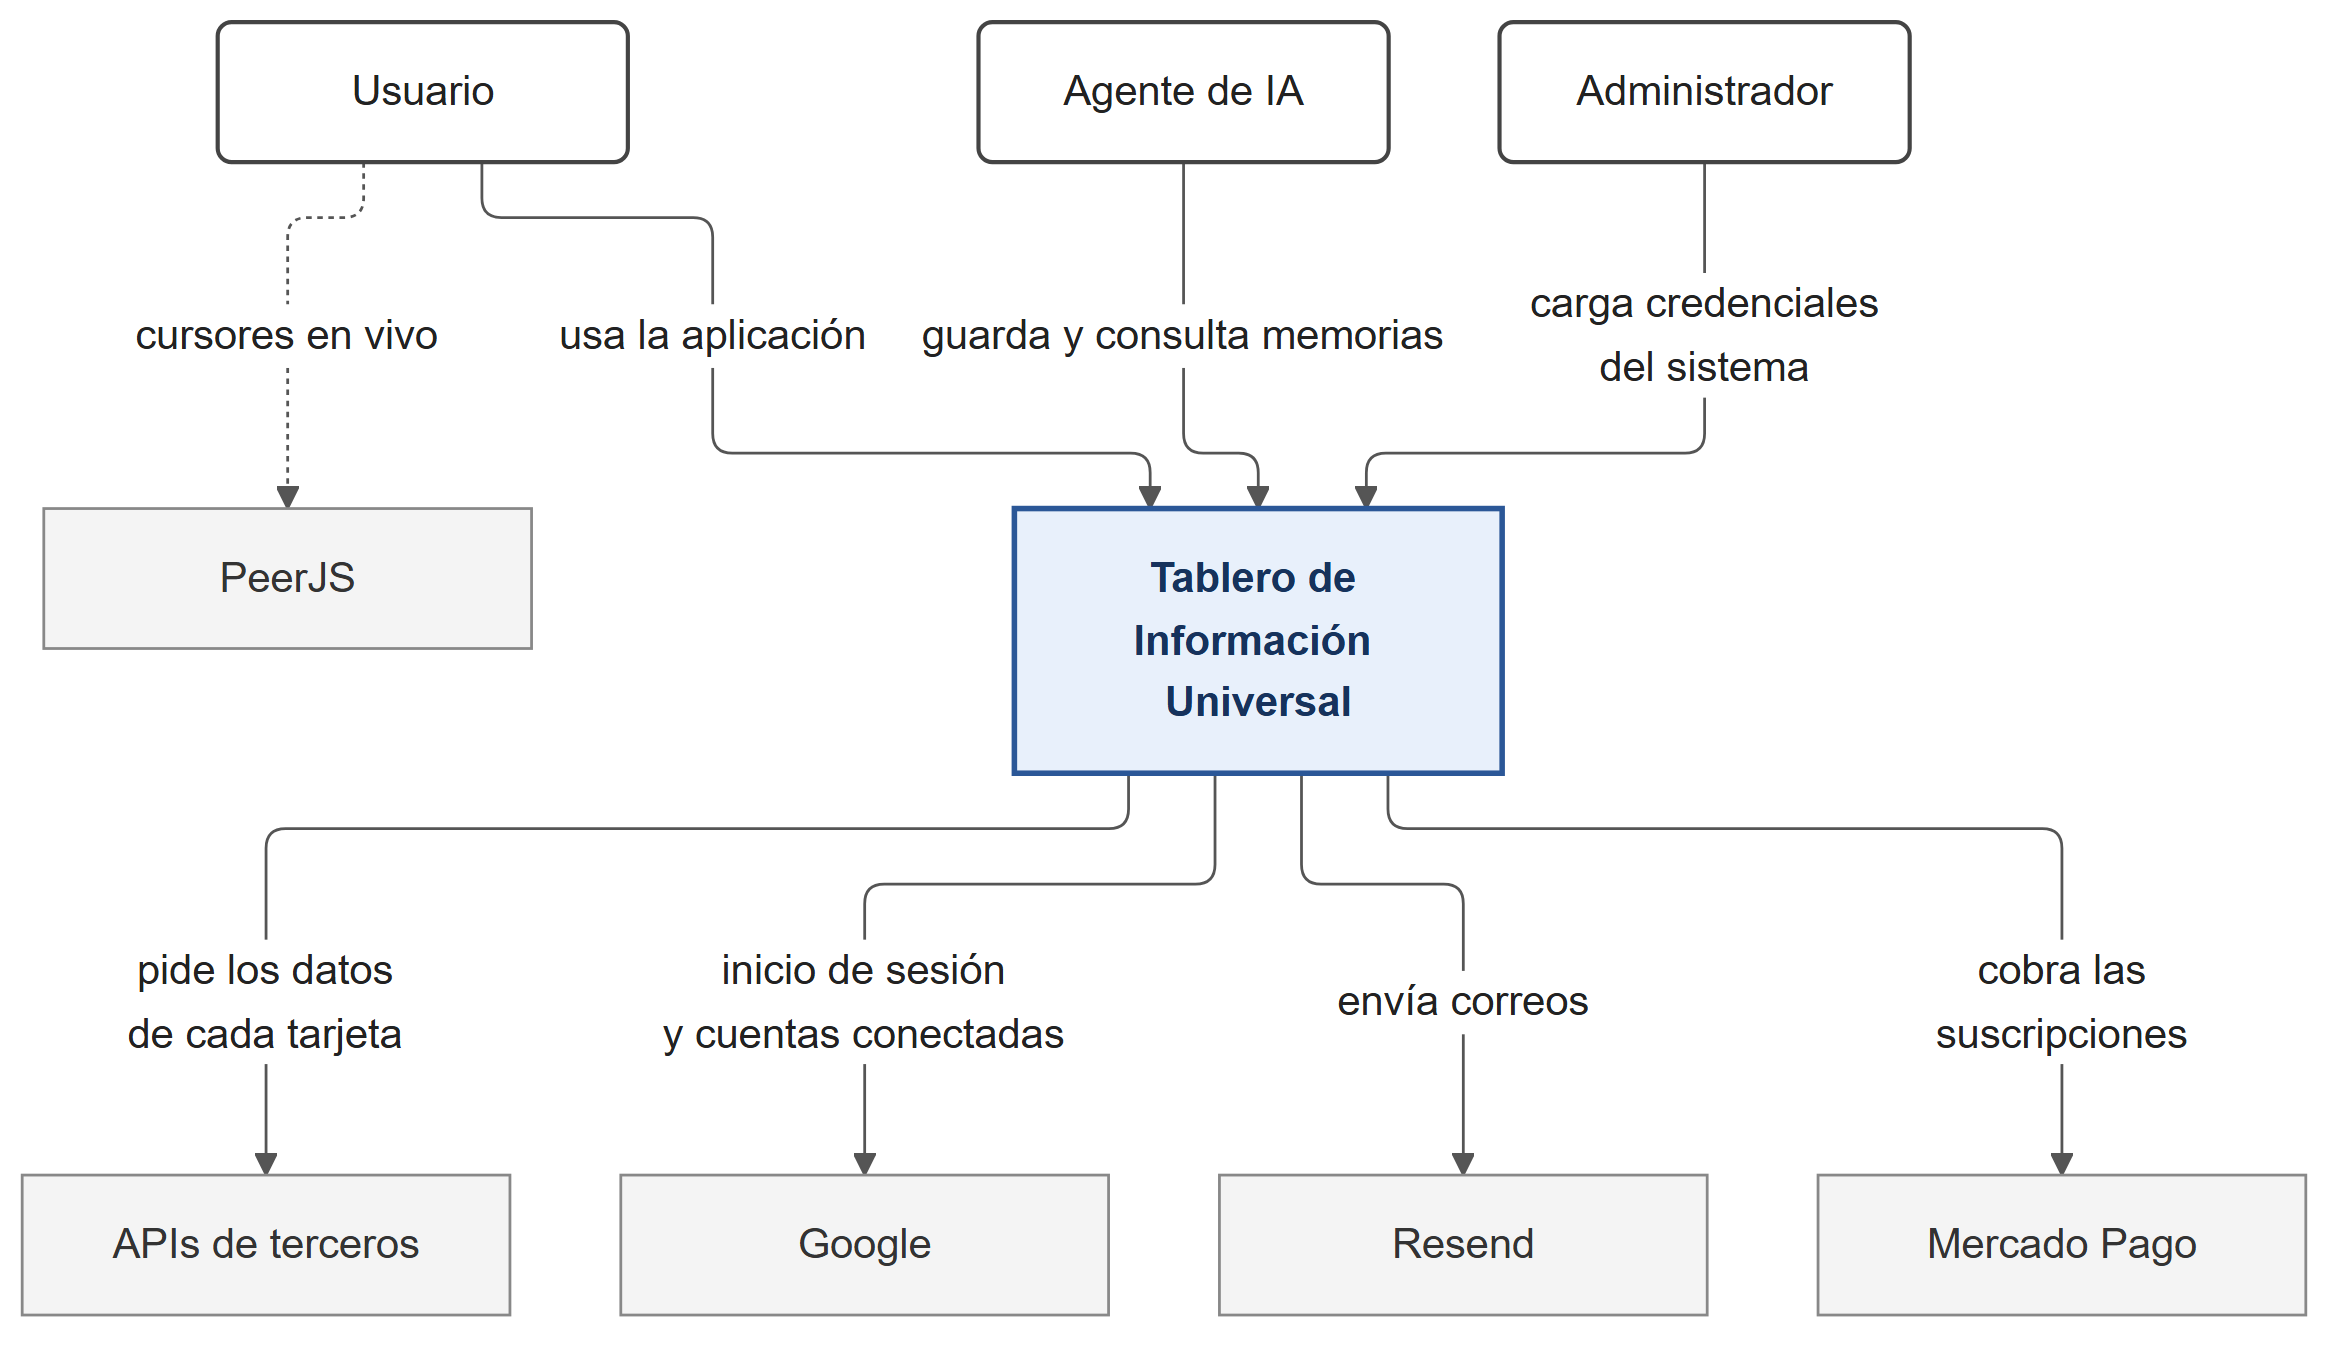
\includegraphics[width=0.92\textwidth]{figuras/fig04.png}
  \caption{Diagrama de contexto}
  \label{fig:diagrama_contexto}
\end{figure}

En la Figura~\ref{fig:diagrama_servicios} se representa el diagrama de servicios, en el cual se detallan los componentes que conforman el sistema y la forma en la que se comunican. Todos los servicios se publican detrás de un único origen, y un proxy inverso distribuye cada pedido según el prefijo de su ruta: \texttt{/api} al backend, \texttt{/ws} al servicio de tiempo real, \texttt{/mcp} al servidor MCP y el resto al frontend. El backend es el único servicio que escribe los datos de negocio en MongoDB, utiliza Redis como caché de resultados, almacén de sesiones y registro de límites de frecuencia de solicitudes, y con Mercado Pago crea y modifica las suscripciones a través de su API y maneja webhooks. El servicio de tiempo real no modifica datos: recibe los cambios de la colección de tableros mediante un change stream de MongoDB y consulta al backend el rol de cada usuario que se conecta. De la misma forma, el servidor MCP no accede a las bases de datos, sino que reenvía al backend cada operación del agente con el token del usuario, por lo que se aplican las mismas reglas de autorización que en la aplicación web.

\begin{figure}[H]
  \centering
  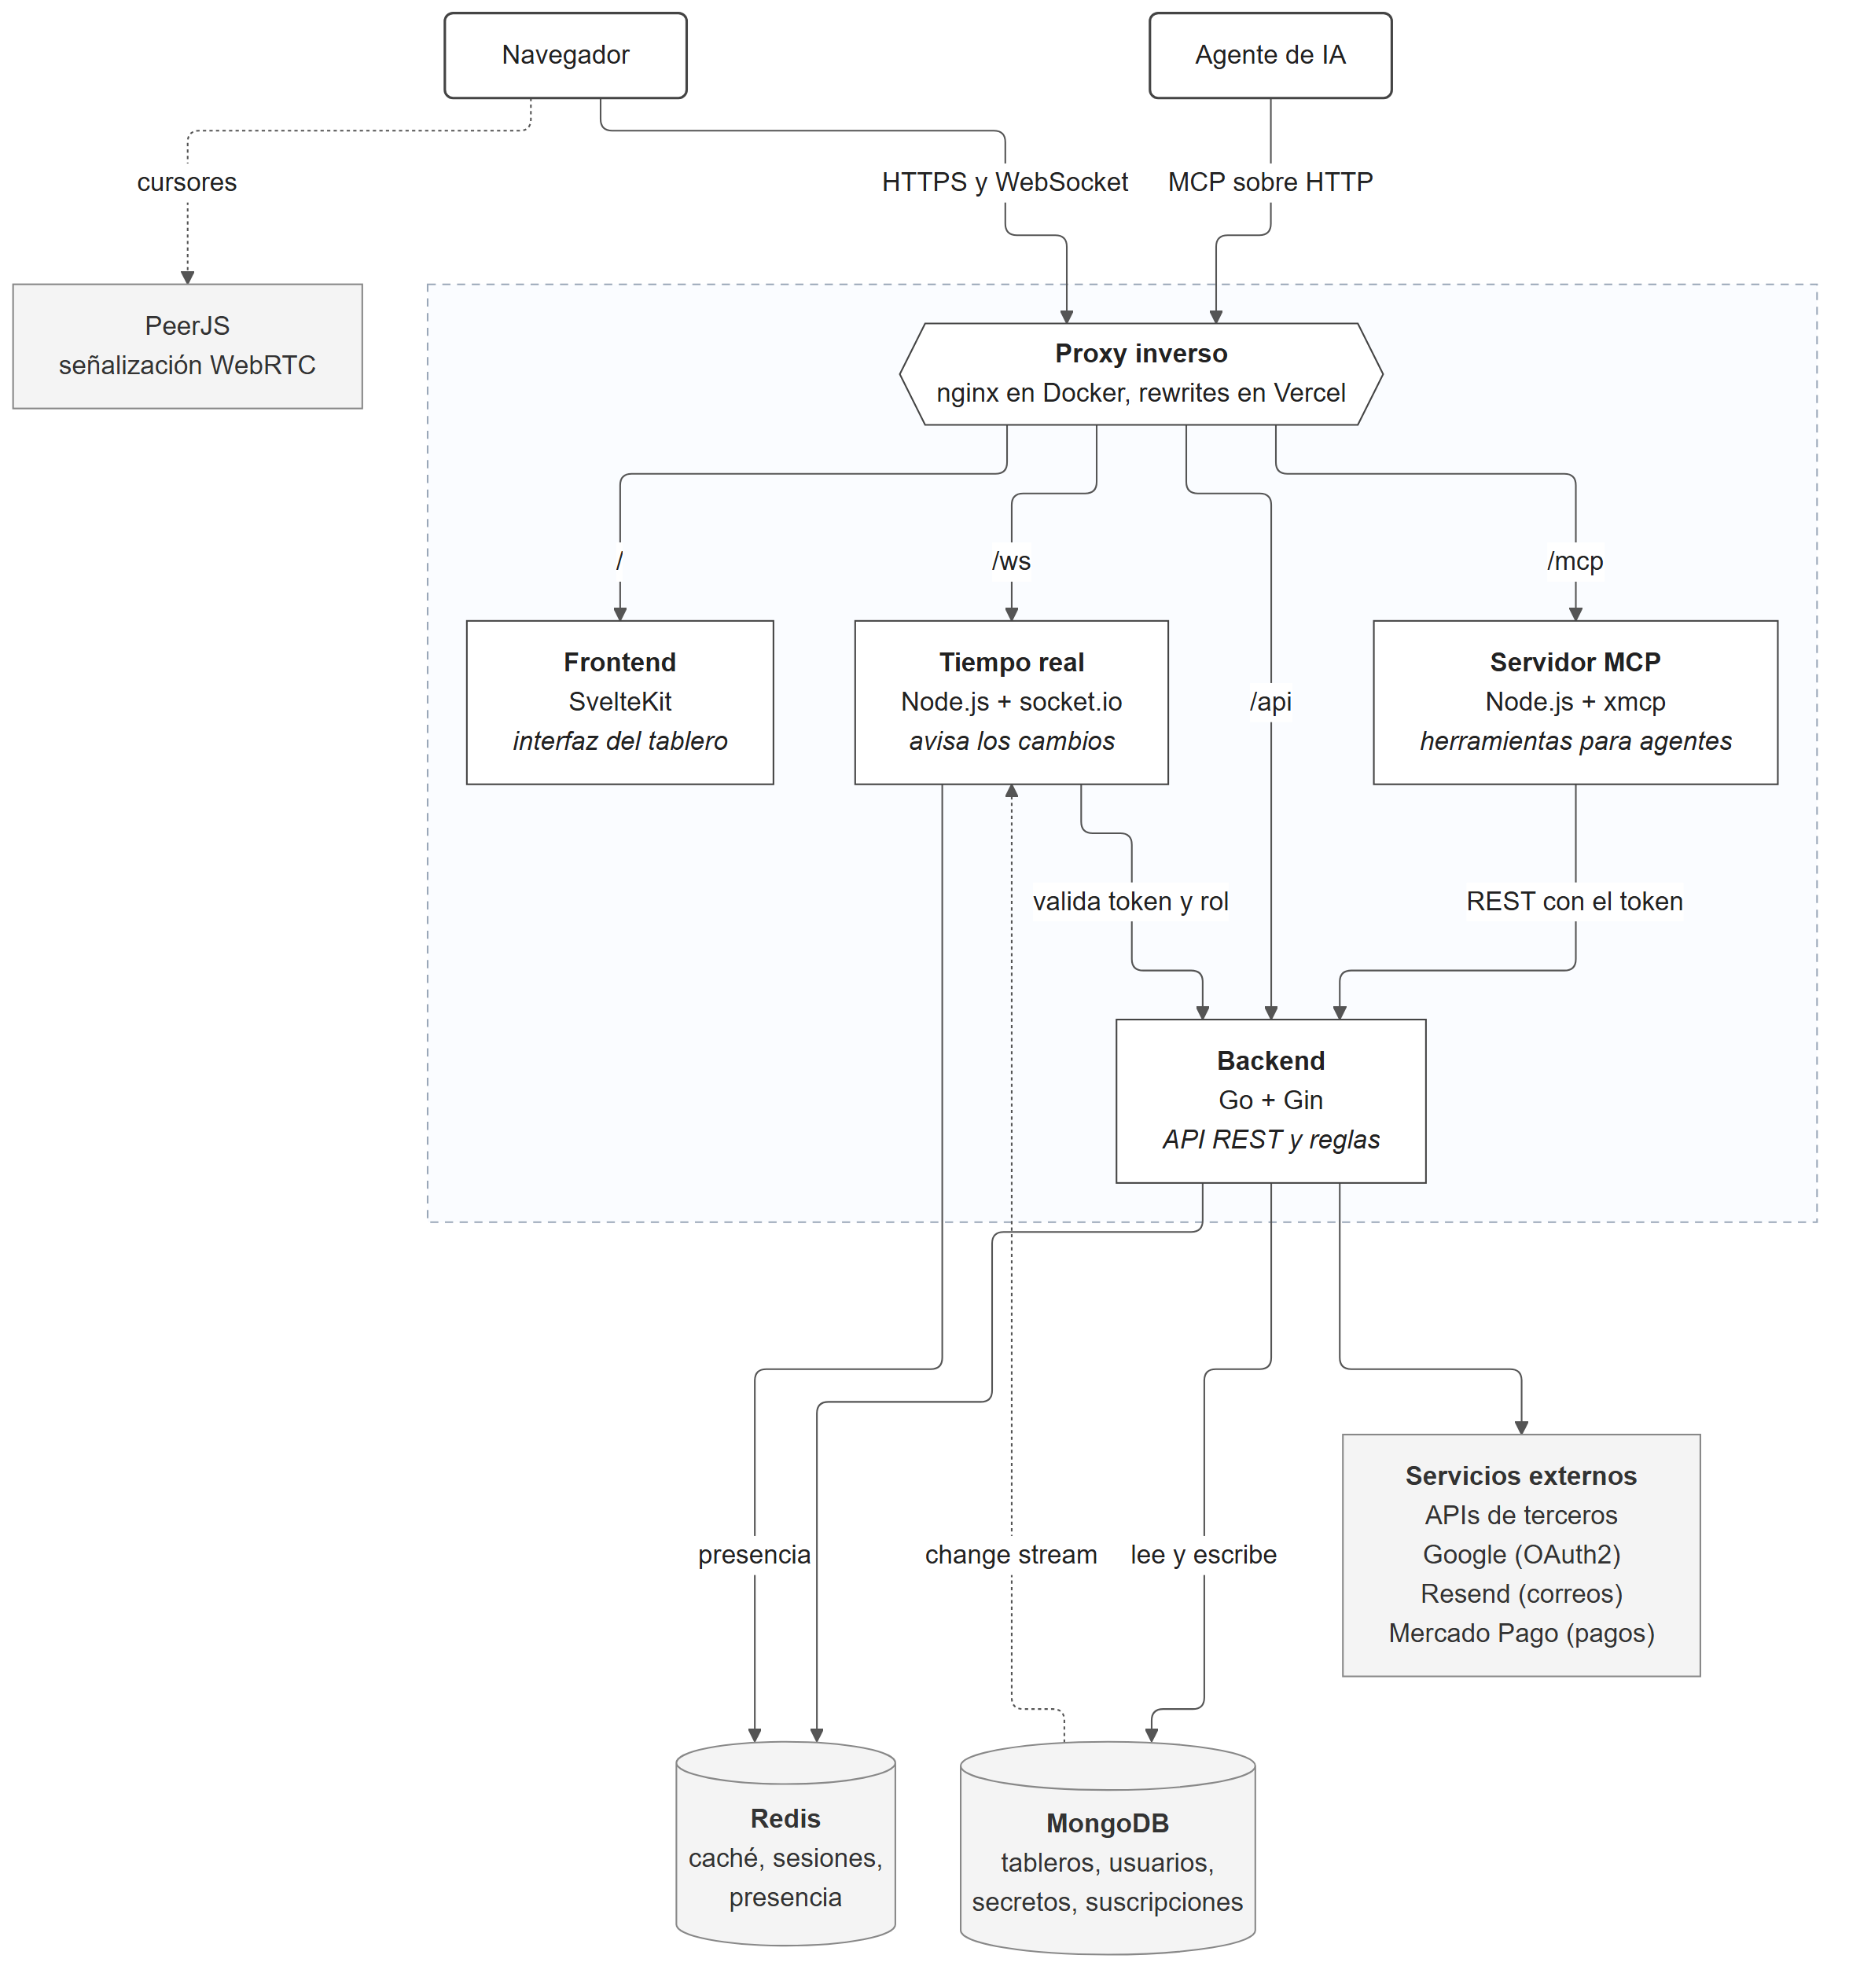
\includegraphics[width=0.92\textwidth]{figuras/fig05.png}
  \caption{Diagrama de servicios}
  \label{fig:diagrama_servicios}
\end{figure}

Para la primera fase de desarrollo del producto, el sistema se despliega en Vercel \cite{vercel_docs}, el cual provee el hosting de la web, las funciones serverless de Go y Node, y el dominio. Para las bases de datos, se utilizan los servicios de MongoDB Atlas \cite{mongodb_docs} y Redis Cloud \cite{redis_docs} respectivamente. El servicio STUN está provisto por PeerJS, el envío de mensajes está gestionado por Resend, y los pagos se procesan con Mercado Pago.

La Figura~\ref{fig:arq_vercel} representa el despliegue en Vercel, en el cual cada carpeta del repositorio se publica como un servicio del mismo proyecto: el frontend con el adaptador de SvelteKit para Vercel, el backend como función de Go, y los servicios de tiempo real y MCP como funciones de Node.js. Las reglas de reescritura del archivo \texttt{vercel.json} cumplen la funcion del proxy inverso, dirigiendo \texttt{/api}, \texttt{/ws} y \texttt{/mcp} a su respectivo servicio y el resto al frontend. Las líneas punteadas representan la variable \texttt{API\_URL}, mediante la cual Vercel les indica a los servicios de tiempo real y MCP la dirección del backend. Servir todo desde un mismo origen evita configurar CORS, permite que la cookie de sesión se envíe con la política \texttt{SameSite=Strict} y hace que una misma compilación del frontend funcione en cualquier dominio, incluidas las URLs de vista previa.

\begin{figure}[H]
  \centering
  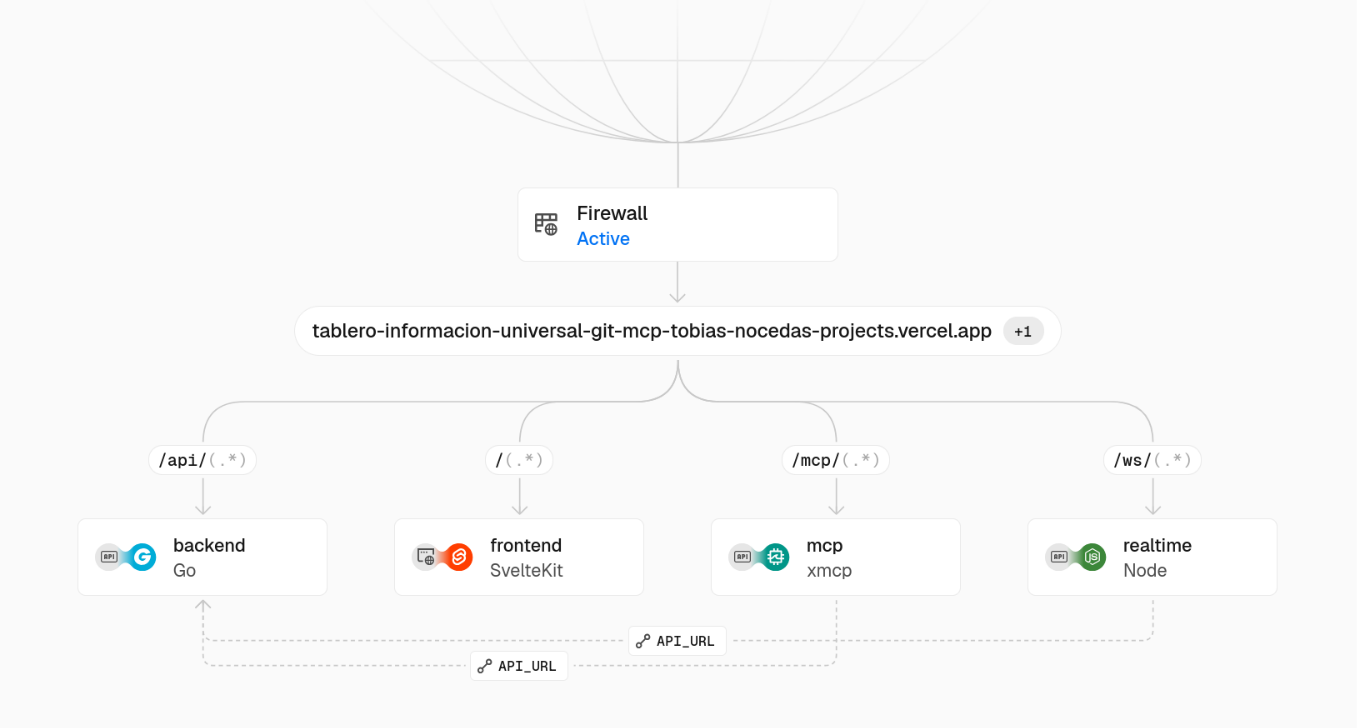
\includegraphics[width=0.95\textwidth]{figuras/fig06.png}
  \caption{Diagrama de arquitectura en Vercel}
  \label{fig:arq_vercel}
\end{figure}

Para el desarrollo local, se utiliza un conjunto de contenedores orquestados con Docker Compose \cite{docker_compose_docs}. Esta separación permite escalar de forma horizontal los componentes que lo requieran (típicamente el backend y el motor de actualización) sin afectar al resto, y simplifica el reemplazo de cualquier pieza individual a medida que el producto evoluciona. La Figura~\ref{fig:arq_docker} representa esta topología de despliegue. El contenedor application load balancer, que ejecuta un servidor Nginx \cite{nginx_docs}, actúa como proxy inverso y cumple la misma función que las reglas de reescritura de Vercel, centralizando el acceso a los distintos servicios. Es el único contenedor que expone un puerto al exterior (80), mientras que MongoDB y Redis permanecen accesibles únicamente desde las redes internas de Docker. MongoDB se configura como un replica set de un único nodo para habilitar el uso de Change Streams.

\begin{figure}[H]
  \centering
  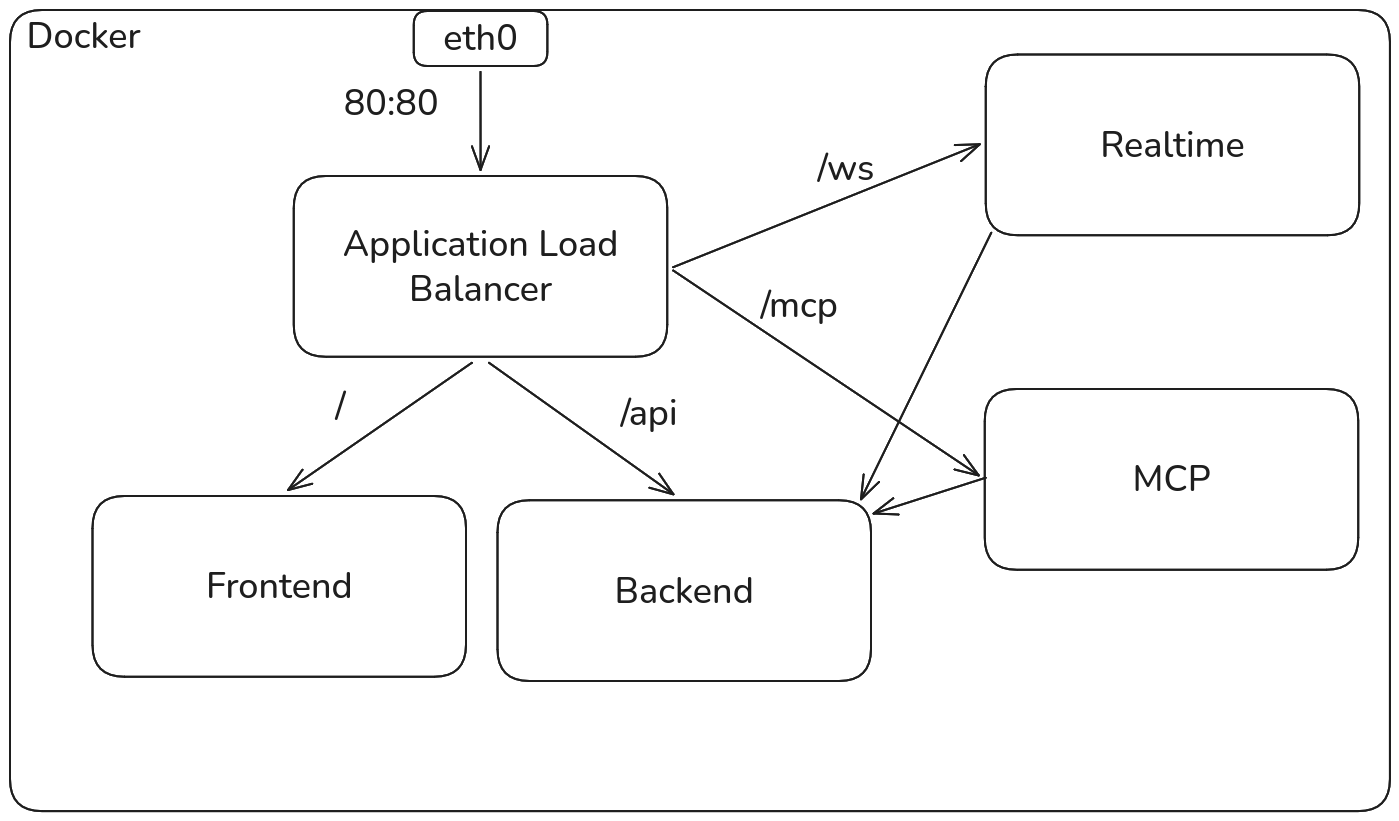
\includegraphics[width=0.9\textwidth]{figuras/fig07.png}
  \caption{Diagrama de arquitectura en Docker}
  \label{fig:arq_docker}
\end{figure}

Como trabajo futuro, se plantea un análisis de costos y del mercado, contemplando el escalamiento del producto a medida que aumenta la adopción del mismo, con el objeto de predecir las necesidades del sistema y los requisitos técnicos de migrar el despliegue según sea rentable.

La Figura~\ref{fig:arq_aws} es una propuesta de arquitectura de despliegue del sistema sobre AWS, que no se encuentra implementada y se plantea como posible evolución del despliegue actual en Vercel. En ella, el tráfico de los usuarios ingresa a través de Route 53 y CloudFront, con Cognito resolviendo la autenticación y WAF la protección perimetral. El frontend estático se sirve desde S3, mientras que la lógica de aplicación se concentra en funciones Lambda que orquestan el acceso a la base de datos, el caché y el motor de integraciones. Esta topología materializa la separación de responsabilidades descrita en la sección anterior y permite escalar de forma independiente cada componente.

\begin{figure}[H]
  \centering
  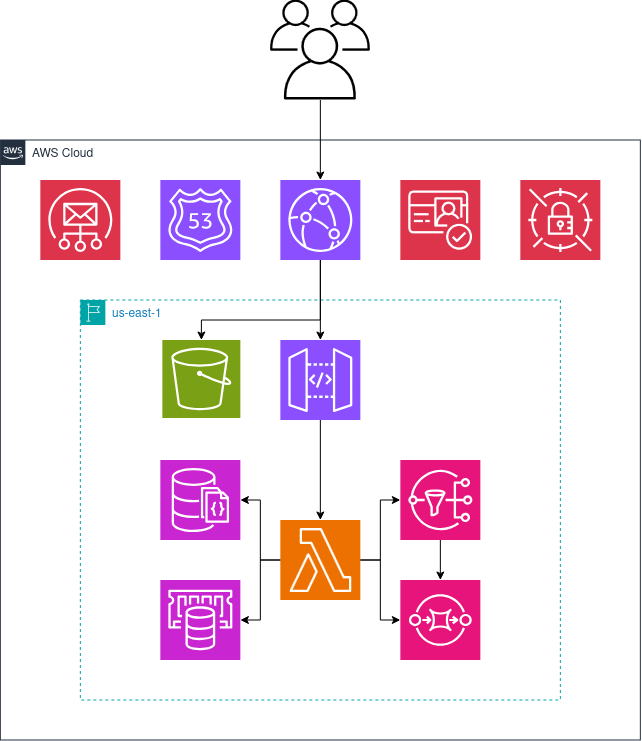
\includegraphics[width=0.82\textwidth]{figuras/fig08.png}
  \caption{Diagrama de arquitectura en AWS}
  \label{fig:arq_aws}
\end{figure}

\section{Flujos de información}
A continuación se describen los principales flujos de información que atraviesan los servicios del sistema, representados mediante diagramas de secuencia.

\subsection{Inicio y la Renovación de Sesión}
La Figura~\ref{fig:seq_sesion} describe el proceso de autenticación y renovación de sesiones. Durante el inicio de sesión, el backend aplica límites de intentos tanto por dirección IP como por cuenta y verifica la contraseña proporcionada mediante Argon2id \cite{rfc9106}. Si la autenticación es exitosa, el backend entrega un token de acceso con una vigencia de 15 minutos y genera un token de refresco, que almacena en Redis y envía al frontend mediante una cookie HttpOnly.

El frontend conserva el token de acceso únicamente en memoria y lo utiliza para autenticar las solicitudes posteriores. Cuando recibe una respuesta HTTP 401, intenta renovar la sesión una única vez, enviando la cookie de refresco al backend. Si la renovación es exitosa, el frontend recibe un nuevo token de acceso y luego reintenta la solicitud original.

En cada renovación, el backend rota el token de refresco y actualiza su registro en Redis. Si detecta que un token de refresco anterior vuelve a utilizarse una vez transcurrido el período de gracia de 10 segundos, revoca toda la familia de sesiones asociada.

\begin{figure}[H]
  \centering
  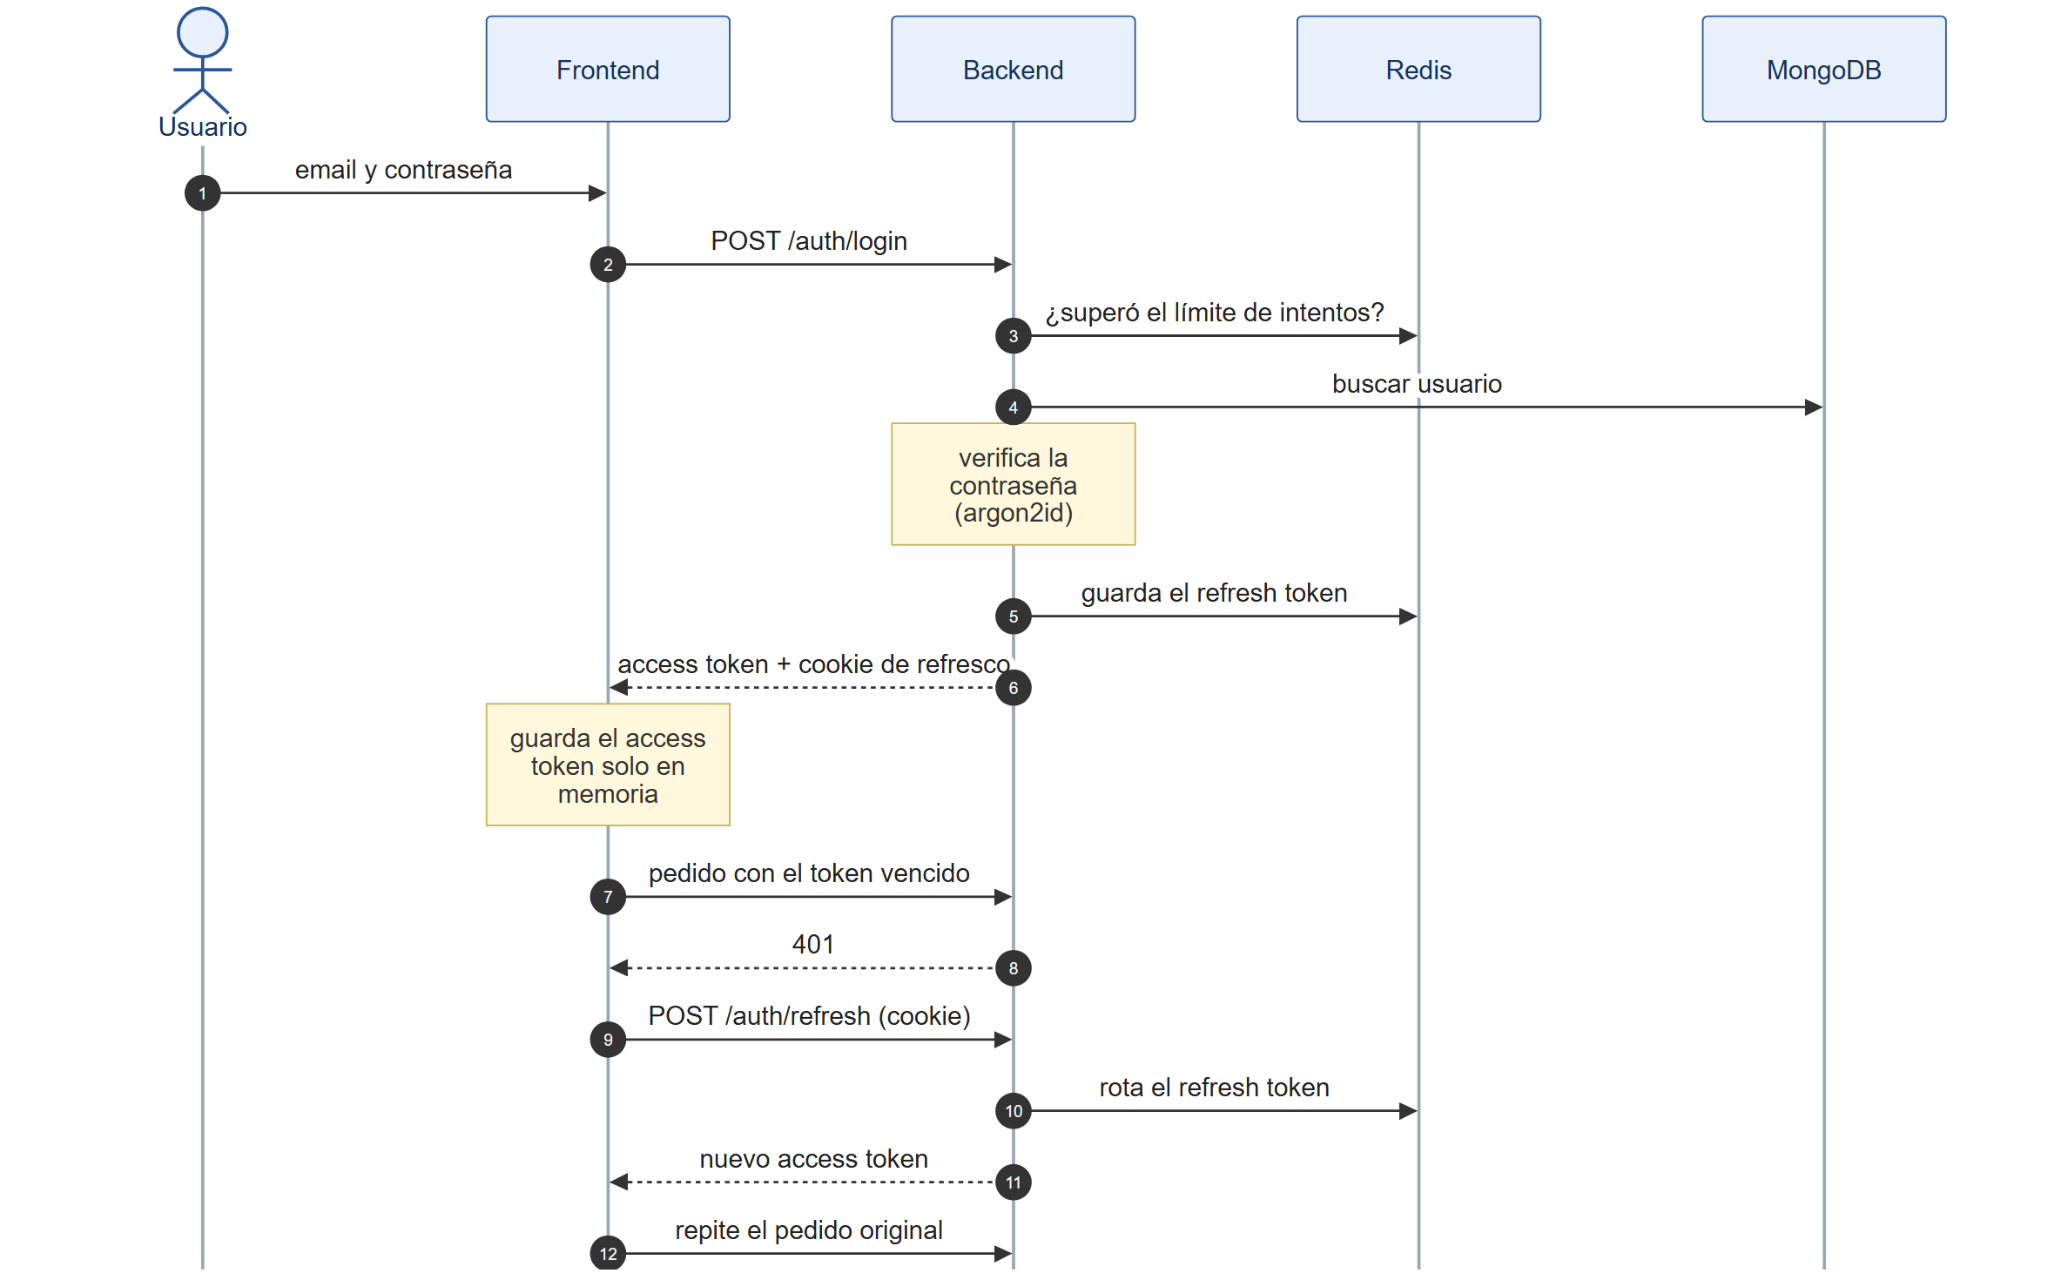
\includegraphics[width=0.95\textwidth]{figuras/fig09.png}
  \caption{Diagrama de secuencia del inicio y la renovación de sesión}
  \label{fig:seq_sesion}
\end{figure}

\subsection{Ejecución de una tarjeta}
La Figura~\ref{fig:seq_ejecucion} ilustra el flujo de ejecución de una tarjeta, uno de los procesos centrales del producto. Ante una solicitud del frontend, el backend verifica que el usuario tenga, como mínimo, el rol de lector sobre el tablero y consulta Redis para determinar si existe un resultado previamente almacenado en caché.

Si no encuentra un resultado, resuelve las credenciales referenciadas por la tarjeta mediante \texttt{\$TOKEN}, utilizando la identidad del usuario indicado en \texttt{RunAs} y verificando que dichas credenciales continúen siendo válidas. Luego, entrega la configuración de la tarjeta al motor de integraciones, que realiza la petición HTTP mediante un cliente que bloquea el acceso a direcciones internas y limita la respuesta a 2 MB y diez segundos. Una vez obtenida la respuesta, el motor la interpreta como JSON o HTML, según el valor del campo \texttt{response}, y aplica la consulta definida en la tarjeta.

Finalmente, el resultado se almacena en Redis durante la cantidad de segundos indicada en \texttt{rate}, con un piso que depende del plan de quien paga el tablero, de manera que las solicitudes posteriores puedan reutilizarlo sin necesidad de volver a consultar la API externa. En el plan Max, el usuario puede además forzar una actualización, que ignora el caché, como máximo una vez cada diez segundos por tarjeta. En el diagrama, el fragmento \texttt{alt} representa los dos caminos posibles del flujo, según exista o no un resultado disponible en caché.

\begin{figure}[H]
  \centering
  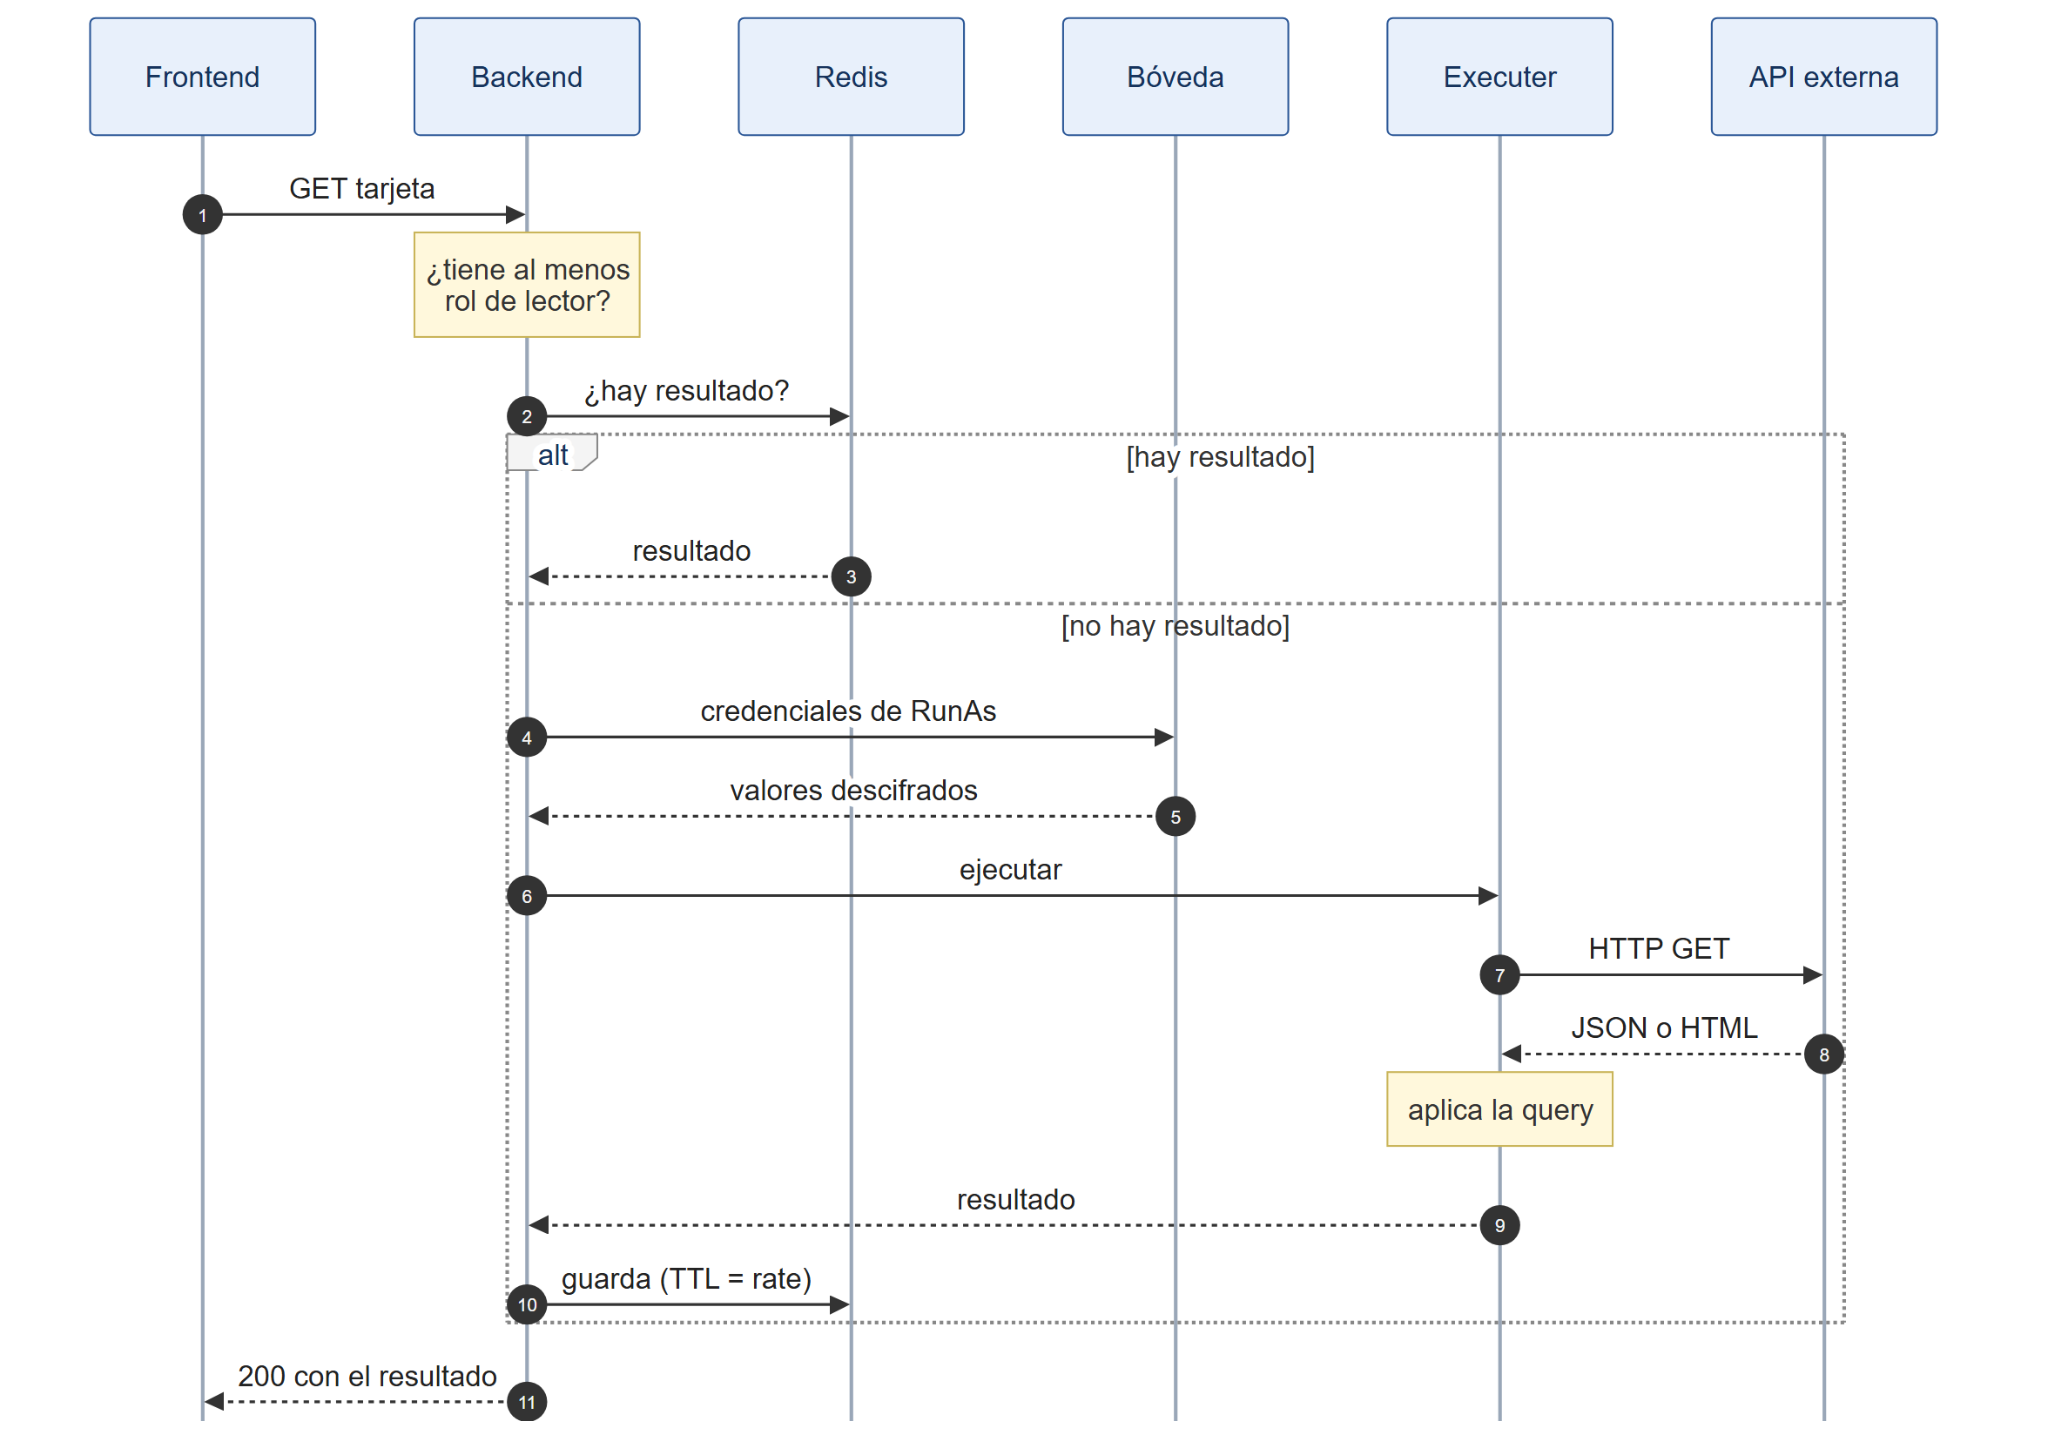
\includegraphics[width=0.95\textwidth]{figuras/fig10.png}
  \caption{Diagrama de secuencia de la ejecución de una tarjeta}
  \label{fig:seq_ejecucion}
\end{figure}

\subsection{Edición Colaborativa en Tiempo Real}
El mecanismo de edición colaborativa en tiempo real se diagramó en la Figura~\ref{fig:seq_realtime} y se desarrolla a través de dos canales de comunicación independientes.

Cuando un usuario abre un tablero, el frontend establece una conexión con el servicio de tiempo real y le proporciona su token de acceso. El servicio de tiempo real utiliza ese token para consultar al backend y verificar los permisos del usuario sobre el tablero. Una vez autorizada la conexión, registra la presencia del usuario en Redis y le envía la lista de participantes conectados. A partir de esta información, los navegadores establecen conexiones WebRTC entre sí, mediante las cuales comparten cursores y movimientos de arrastre directamente, sin que estos datos deban pasar por el servidor.

Por otro lado, cuando un usuario con permisos de edición modifica el tablero, el backend persiste los cambios en MongoDB. El servicio de tiempo real escucha directamente el Change Stream de la colección de tableros, configurado para recibir únicamente operaciones de actualización. Ante cada modificación, MongoDB proporciona el documento completo del tablero en su estado actualizado. El servicio de tiempo real recibe este evento y distribuye el tablero actualizado a todos los participantes.

Finalmente, un minuto antes del vencimiento del token de acceso, el servicio de tiempo real solicita su renovación y vuelve a verificar los permisos del usuario. Si el usuario fue removido del tablero, el servicio interrumpe su conexión y deja de enviarle actualizaciones. De esta manera, un participante removido pierde el acceso a las actualizaciones en tiempo real a más tardar durante el siguiente proceso de renovación del token.

\begin{figure}[H]
  \centering
  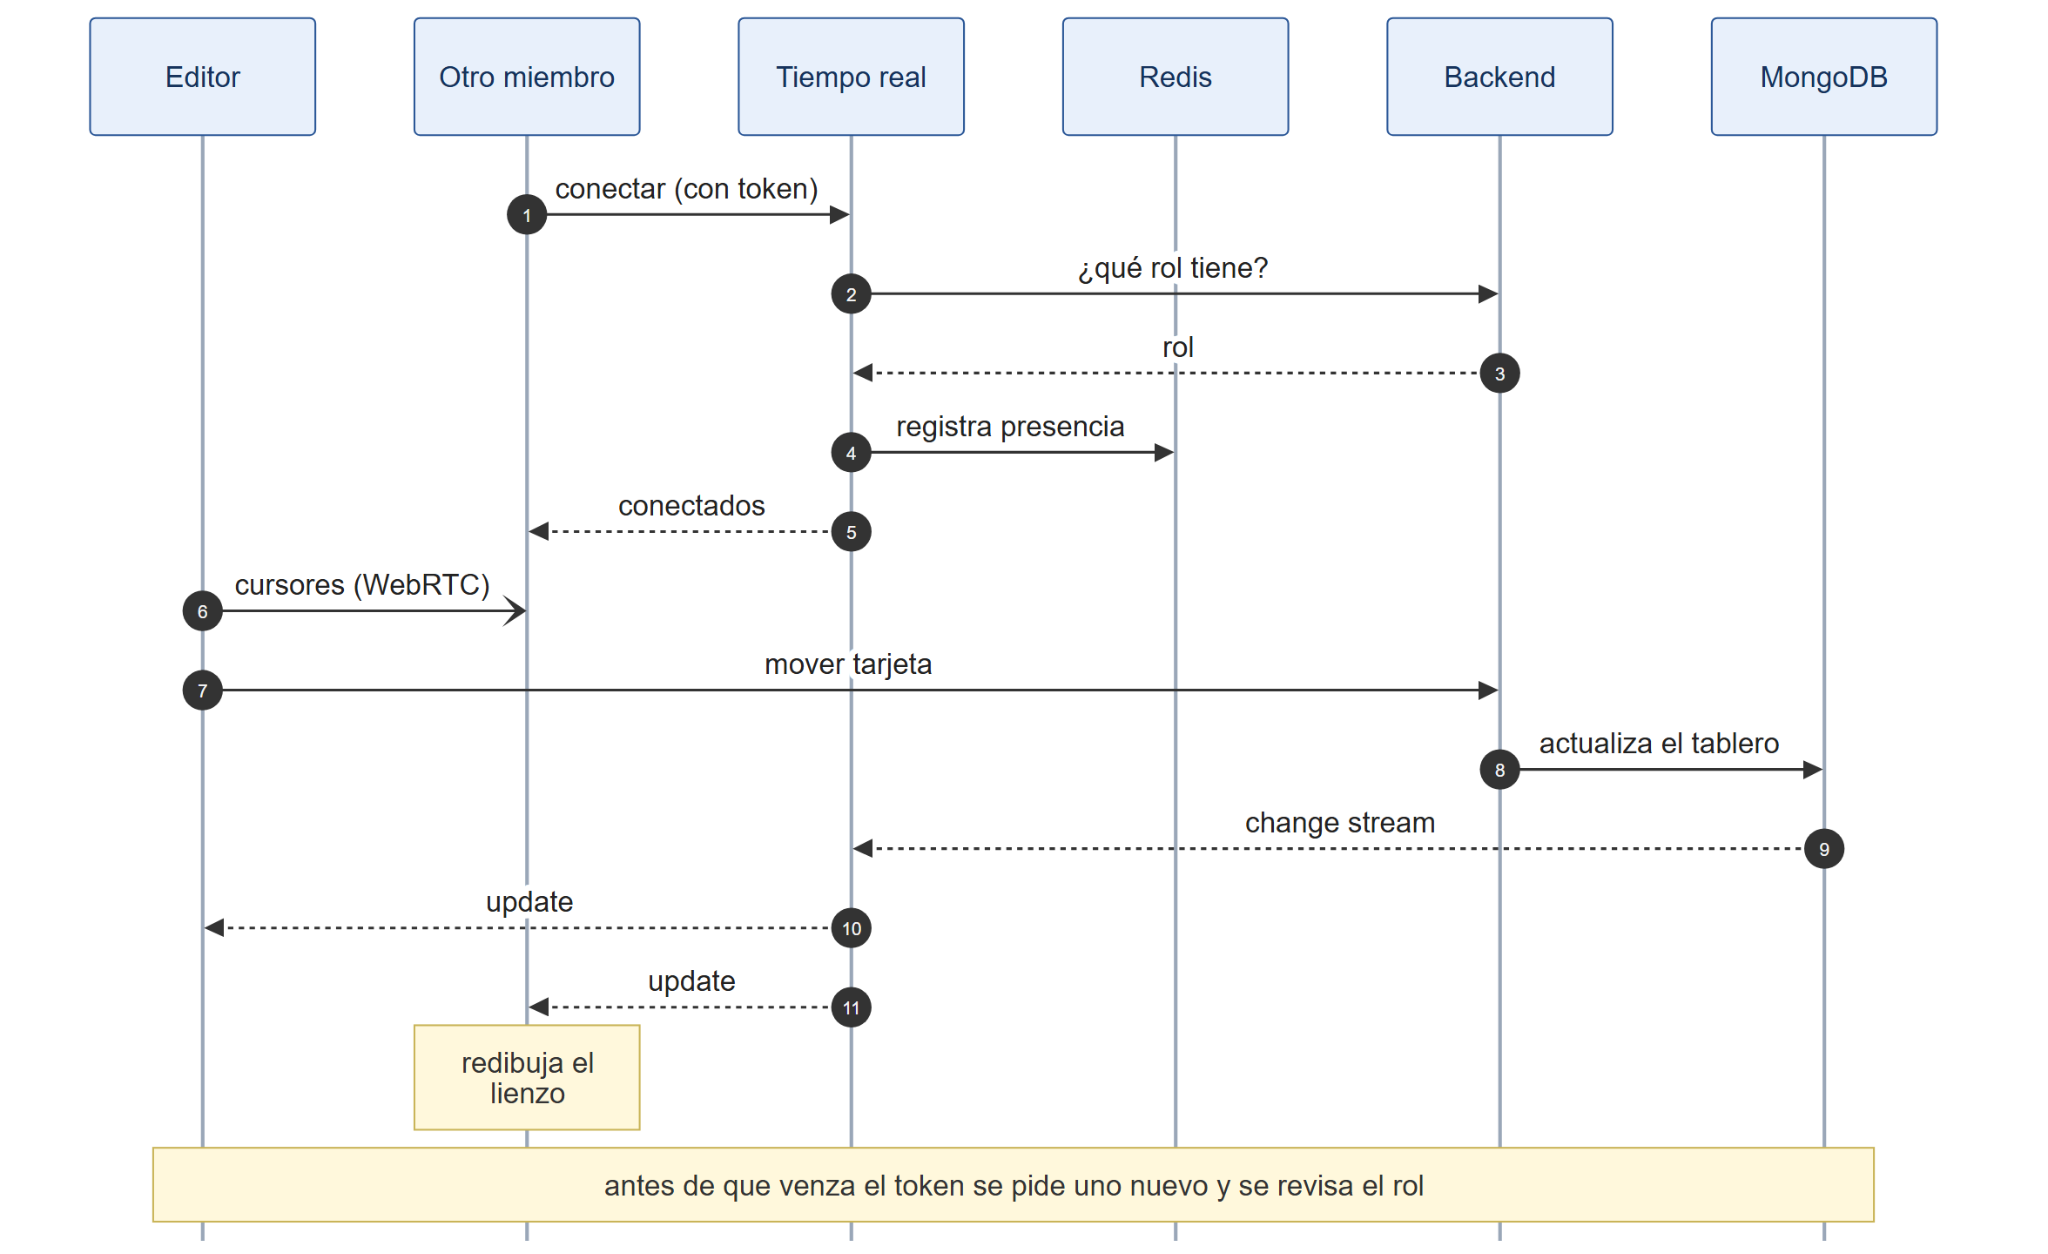
\includegraphics[width=0.95\textwidth]{figuras/fig11.png}
  \caption{Diagrama de secuencia de la edición colaborativa en tiempo real}
  \label{fig:seq_realtime}
\end{figure}

\subsection{Uso de servidor MCP}
La Figura~\ref{fig:seq_mcp} esquematiza la interacción de un agente de inteligencia artificial con el sistema a través del servidor MCP. En primer lugar, el desarrollador genera desde su perfil un token personal (con el prefijo \texttt{tiu\_pat\_}), cuyo vencimiento puede configurarse en 7, 15 o 30 días, cada usuario puede tener hasta diez tokens activos, los cuales nunca se renueva. Por motivos de seguridad, el backend almacena únicamente el hash SHA-256 del token, sin conservar su valor original. El acceso por token es una funcionalidad de los planes pagos.

Para interactuar con el sistema, el agente de IA proporciona el token personal al servidor MCP, que expone las herramientas disponibles y traduce cada invocación en una o más llamadas a la API REST del backend, reenviando el token sin almacenarlo. El servidor presenta cada tablero como un grafo de conocimiento personal, cada tarjeta como una memoria y cada hilo como una asociación entre memorias. Las herramientas permiten listar, crear y eliminar tableros (\texttt{list\_pkgs}, \texttt{create\_pkg} y \texttt{delete\_pkg}), listar las memorias de un tablero (\texttt{memories}), guardar una memoria de texto (\texttt{consolidate}), modificarla (\texttt{reconsolidate}) y eliminarla (\texttt{forget}), y vincular memorias o desvincularlas (\texttt{associate} y \texttt{dissociate}), nombrando la relación y su dirección. La herramienta \texttt{perceive} guarda una memoria viva: una tarjeta personalizada que consulta una API o una página web mediante \texttt{GET} o \texttt{POST} y se actualiza periódicamente. Las credenciales nunca pasan por el agente, que las referencia como \texttt{\$NOMBRE} para que el backend las resuelva desde la bóveda del tablero. Finalmente, \texttt{retrieve} recupera una memoria con sus datos actualizados, cómo se obtienen si es una memoria viva y las memorias relacionadas, indicando la dirección y la etiqueta de cada relación.

El backend autentica las solicitudes mediante el token personal y las restringe a una lista explícita de rutas: la lectura de tableros, tarjetas, organizaciones, el perfil y el catálogo de integraciones, y la creación, edición y eliminación de tableros, tarjetas e hilos. Cualquier otra ruta, como la gestión de secretos, el uso compartido, los tokens o la facturación, responde 403. Además, aplica los roles que el usuario posee sobre cada tablero, de modo que el agente no puede realizar operaciones que excedan los permisos de su propietario.

\begin{figure}[H]
  \centering
  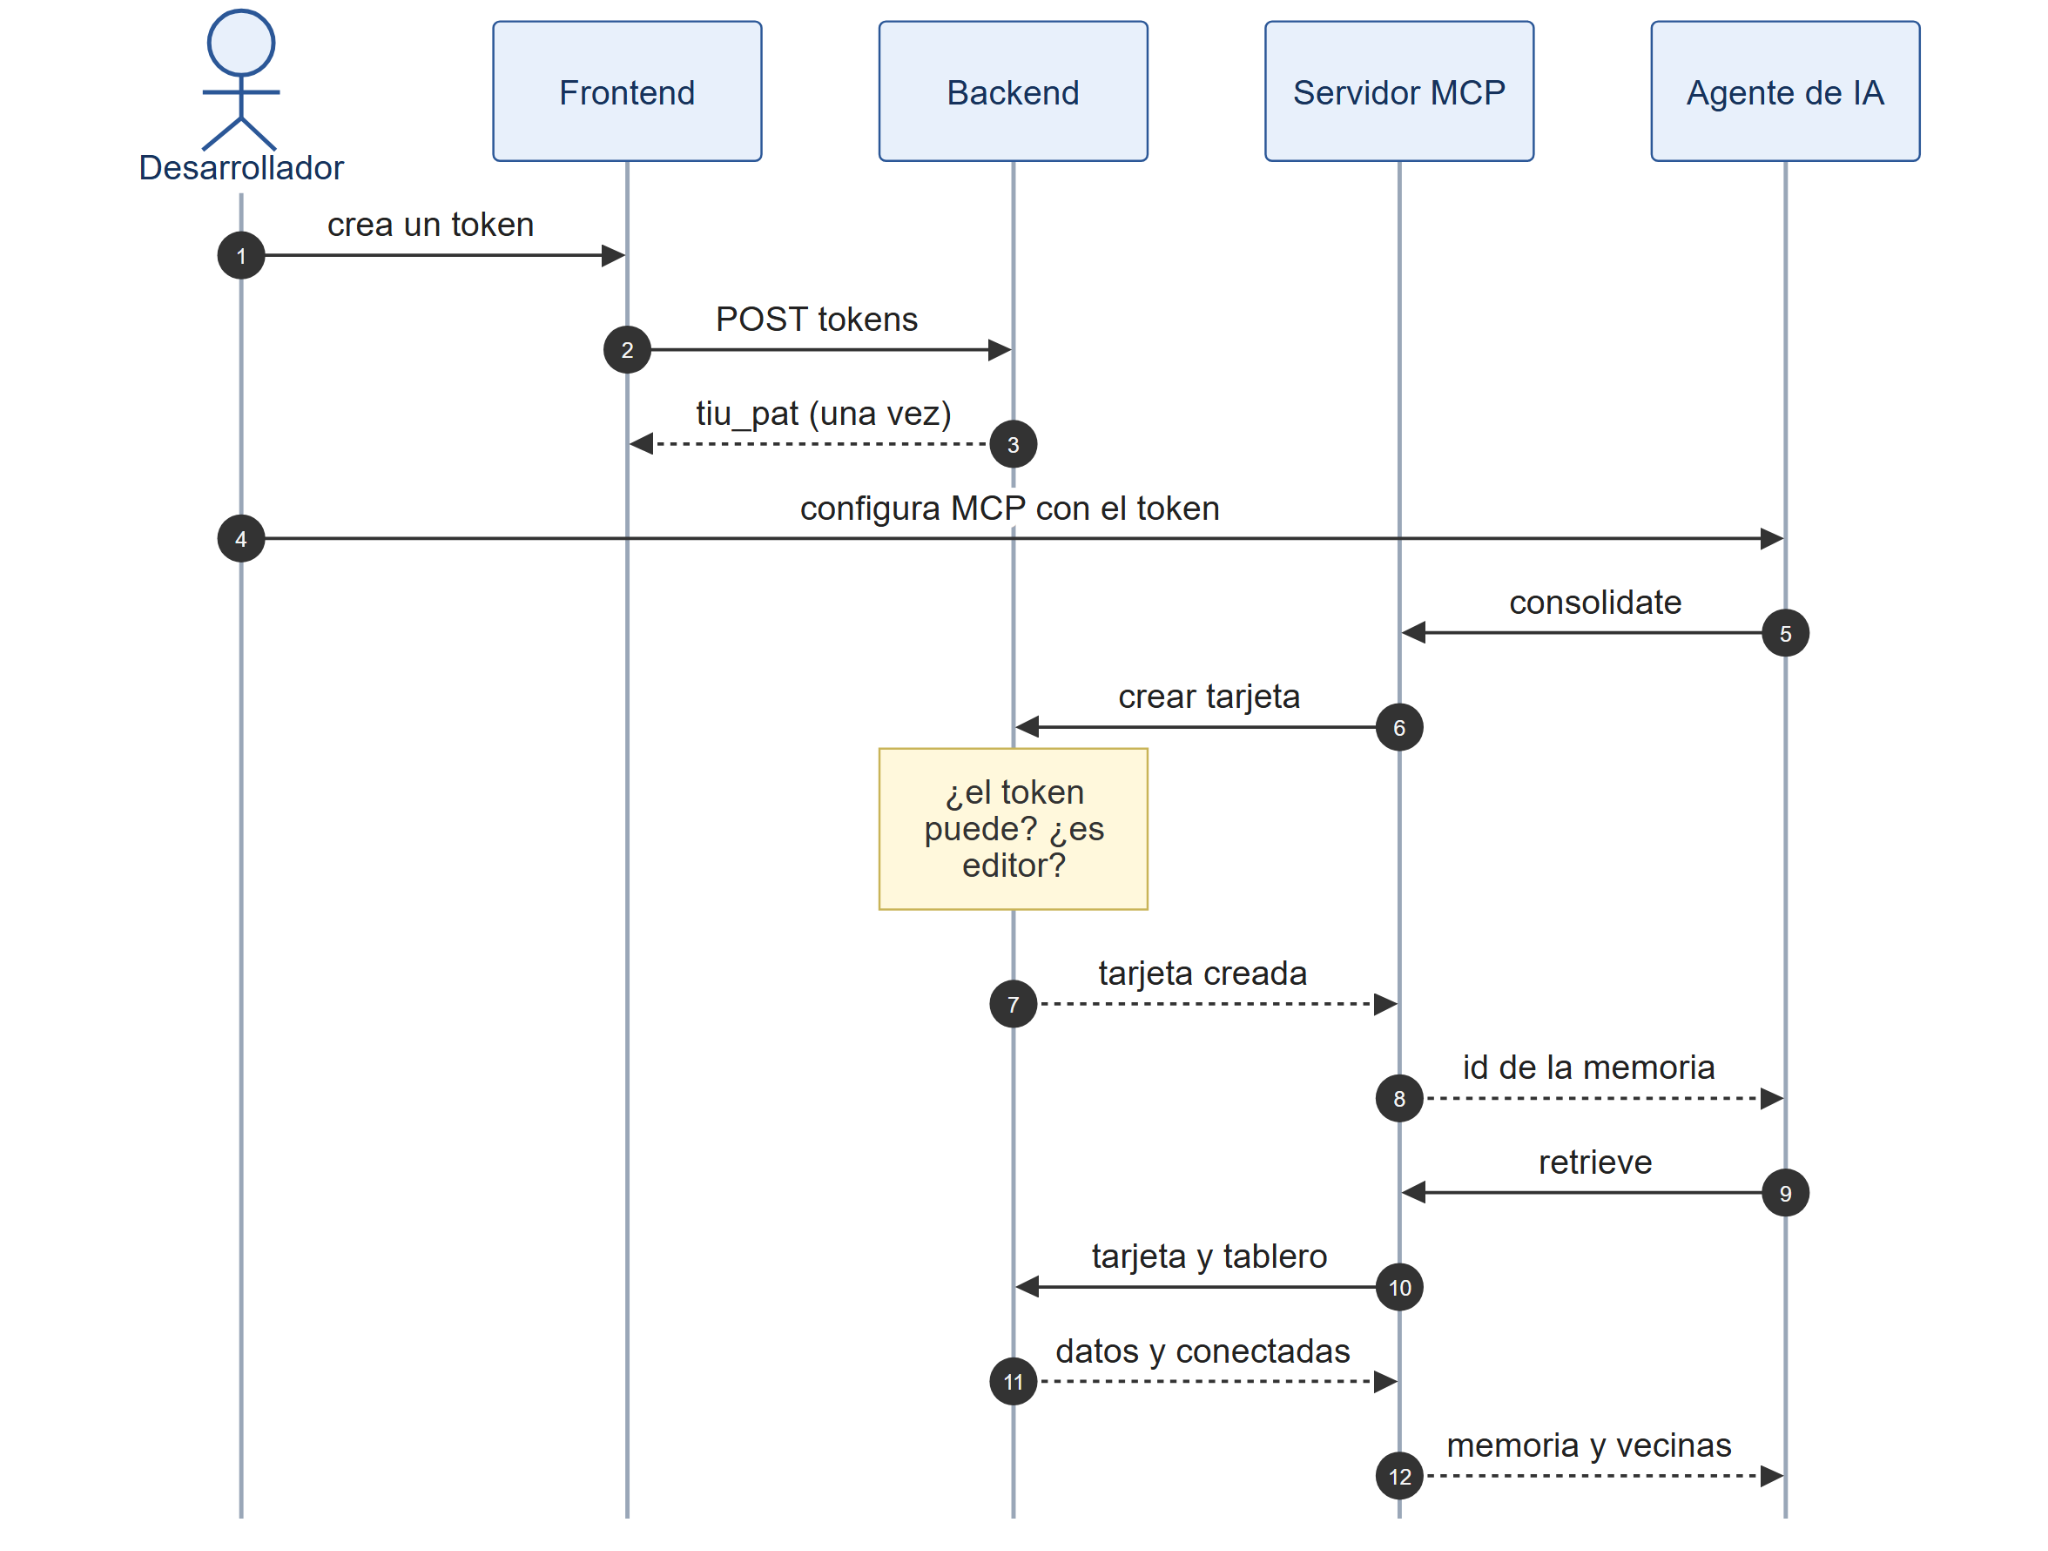
\includegraphics[width=0.95\textwidth]{figuras/fig12.png}
  \caption{Diagrama de secuencia del uso por parte de un agente de IA}
  \label{fig:seq_mcp}
\end{figure}

\subsection{Conexión OAuth2}
La Figura~\ref{fig:seq_oauth2} describe el proceso de vinculación de una cuenta externa mediante OAuth2. En primer lugar, el backend genera la URL de consentimiento y almacena en Redis el estado del intercambio, asociado al usuario que inició el proceso. Luego, el proveedor OAuth2 redirige al frontend con el código de autorización, que este reenvía al backend para completar el intercambio.

Al recibir el código, el backend verifica que el usuario que intenta completar el proceso sea el mismo que lo inició. Si la validación es satisfactoria, el backend intercambia el código por los correspondientes tokens de acceso y los almacena cifrados mediante la clave de datos del ámbito seleccionado. En ningún momento los tokens son enviados al frontend.

\begin{figure}[H]
  \centering
  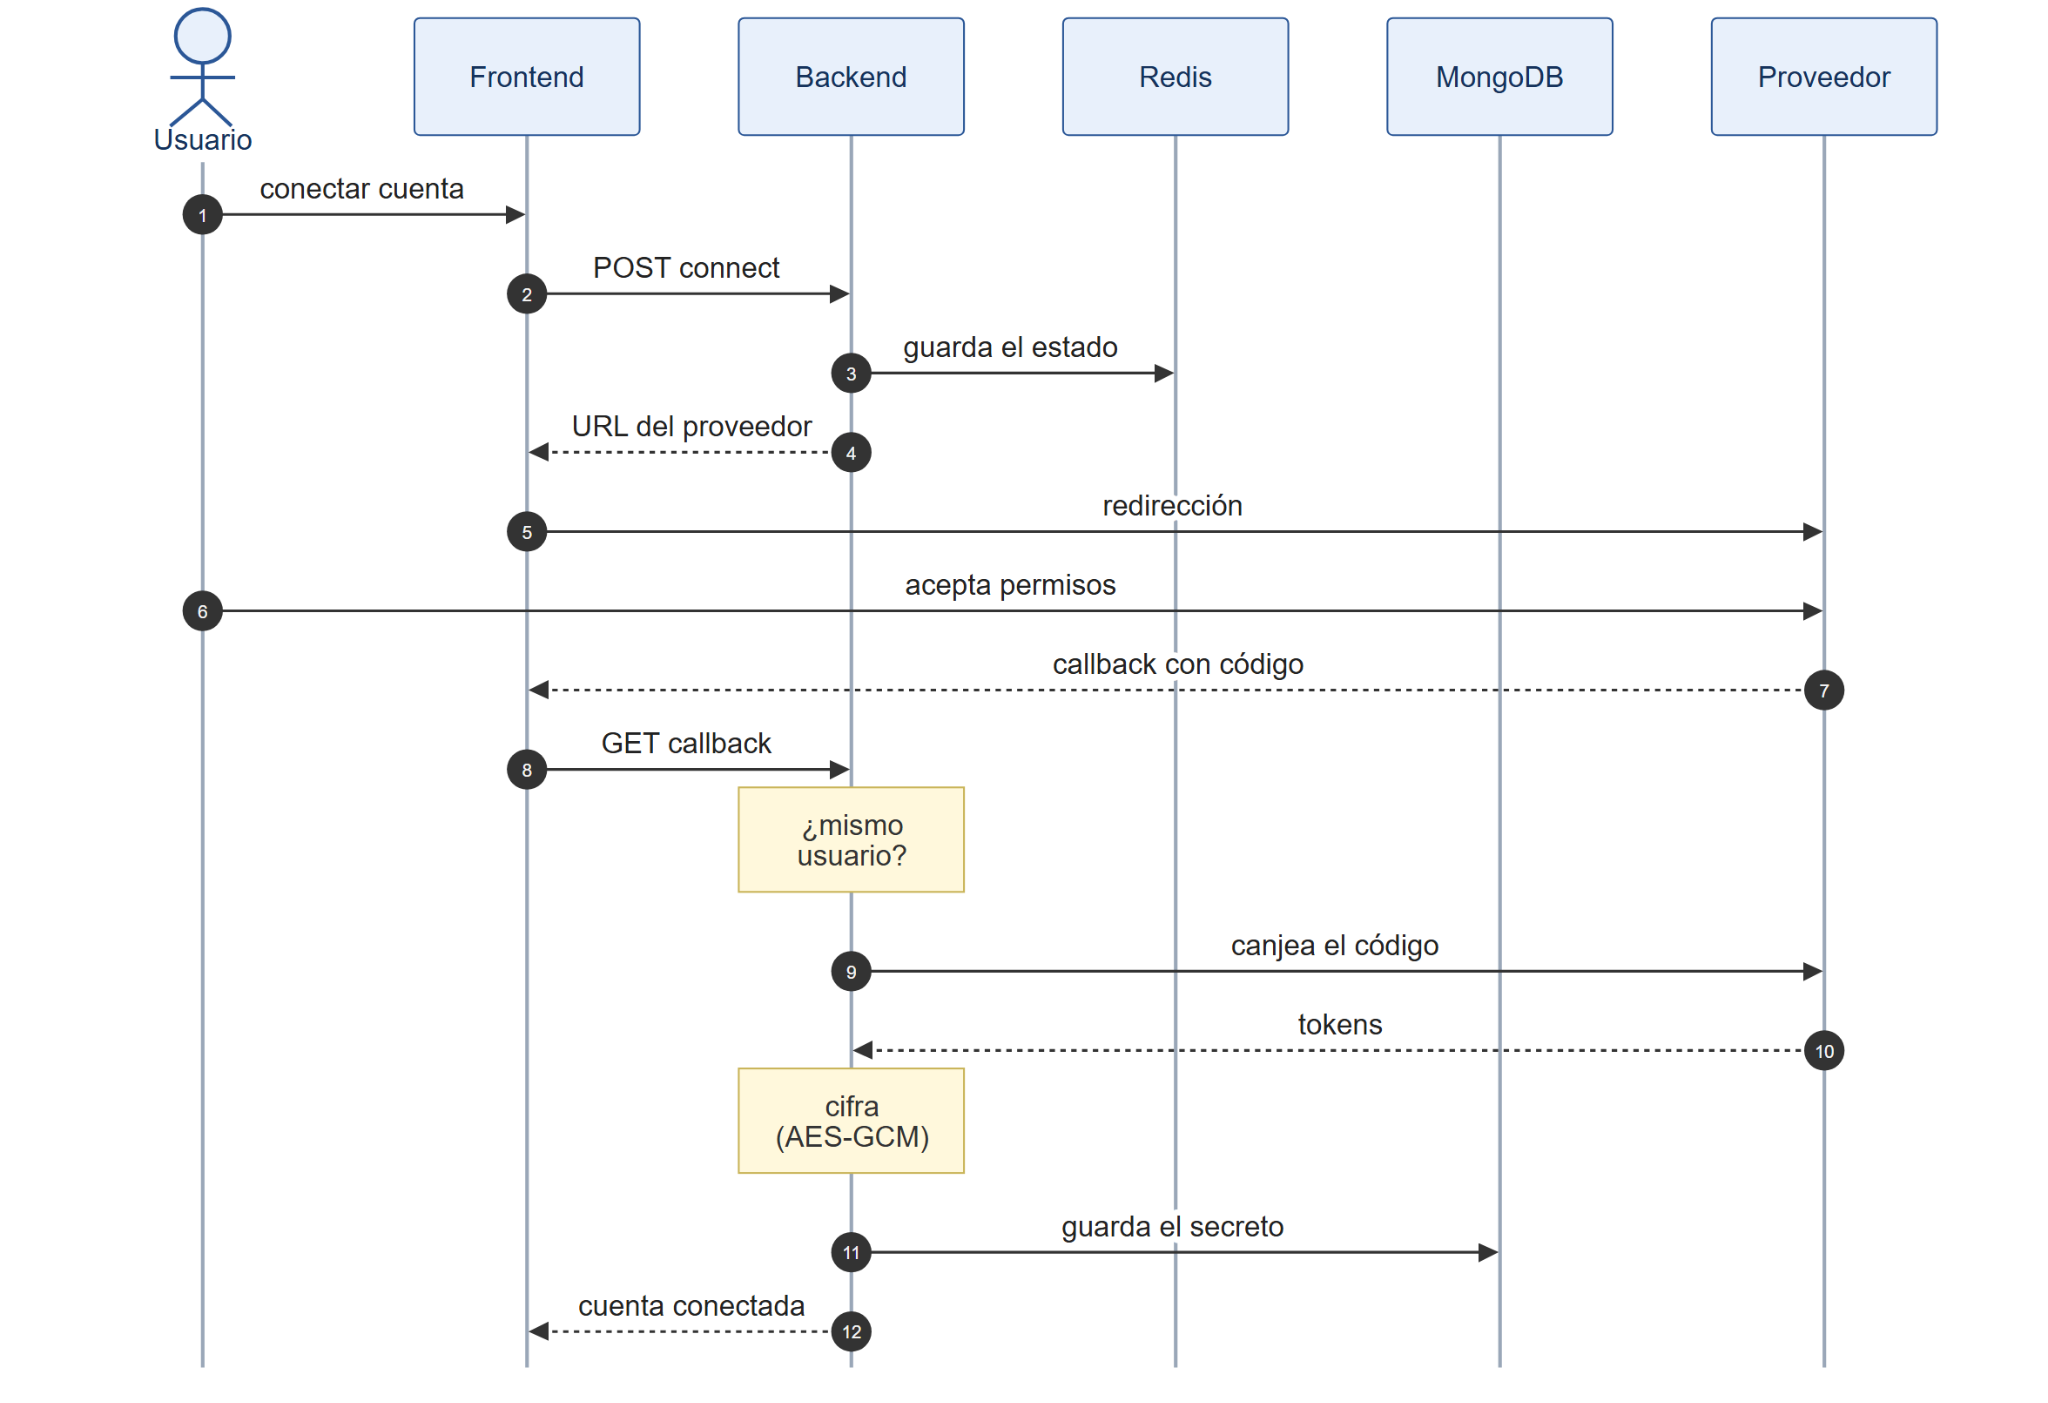
\includegraphics[width=0.95\textwidth]{figuras/fig13.png}
  \caption{Diagrama de secuencia de la conexión de una cuenta mediante OAuth2}
  \label{fig:seq_oauth2}
\end{figure}

\section{Diseño de la base de datos}
A continuación se detallan las colecciones principales de MongoDB. Para cada campo se especifica su tipo físico BSON, si se encuentra indexado y una breve descripción de su propósito, indicando cuando corresponde si se trata de una referencia a otra colección o de un objeto embebido.

\subsection{Colección: boards}
La siguiente colección almacena la metadata del tablero, sus miembros con el rol de cada uno, las relaciones visuales entre elementos (strands) y una lista optimizada de los post-its activos.

\begin{tablacoleccion}{Colección \texttt{boards} MongoDB}{tab:col_boards}
  \_id & binData (UUID) & Sí (Primary) & Identificador único del tablero. \\
  name & string & No & Nombre visible del tablero. \\
  owner & string & Sí & ID del usuario creador (referencia a \texttt{users}). \\
  members & array (objects) & Sí (\texttt{members.user}) & Usuarios con acceso al tablero, cada uno con su rol. \\
  members[].user & string & Sí & ID del miembro (referencia a \texttt{users}). \\
  members[].role & string & No & Rol del miembro: \texttt{editor} o \texttt{viewer}. \\
  org & binData (UUID) & Sí & Organización a la que pertenece el tablero (referencia a \texttt{orgs}). Opcional. \\
  postits & array (objects) & No & Estructura embebida con datos de renderizado de los post-its. Los campos de estilo de cada tarjeta son opcionales y un valor por defecto no se almacena. \\
  postits[].id & binData (UUID) & No & ID de la configuración completa en la colección \texttt{postit}. \\
  postits[].type & string & No & Clave de la integración o plantilla de la que proviene la tarjeta (vacía en una tarjeta personalizada); el frontend la usa para elegir cómo dibujarla. \\
  postits[].title & object & No & Título de la tarjeta (\texttt{text}) y si interpola variables del resultado (\texttt{vars}). \\
  postits[].position & object & No & Coordenadas x/y de la tarjeta dentro del lienzo. \\
  postits[].color & string & No & Color de fondo de la tarjeta: la paleta de los hilos o \texttt{white}. Opcional. \\
  postits[].border & string & No & Borde de la tarjeta: \texttt{none}, \texttt{solid}, \texttt{dashed} o \texttt{dotted}. Opcional. \\
  postits[].border\_width & string & No & Grosor del borde: \texttt{thin}, \texttt{normal} o \texttt{thick}. Opcional. \\
  postits[].border\_color & string & No & Color del borde, con las mismas opciones que \texttt{color}; si falta, sigue el color de la tarjeta. Opcional. \\
  postits[].text\_align & string & No & Alineación horizontal del texto: \texttt{left}, \texttt{center} o \texttt{right}. Opcional. \\
  postits[].vertical\_align & string & No & Ubicación vertical del texto: \texttt{top}, \texttt{middle} o \texttt{bottom}; se nota en una tarjeta con alto propio. Opcional. \\
  postits[].width & double & No & Ancho de la tarjeta en píxeles del lienzo, entre 120 y 1600. Opcional. \\
  postits[].height & double & No & Alto de la tarjeta en píxeles del lienzo, entre 60 y 1200. Opcional. \\
  strands & array (objects) & No & Lista de conexiones o hilos entre post-its. Los campos de estilo de cada hilo son opcionales y un valor por defecto no se almacena. \\
  strands[].id & binData (UUID) & No & Identificador único del hilo. \\
  strands[].source & binData (UUID) & No & Post-it de origen del hilo. \\
  strands[].target & binData (UUID) & No & Post-it de destino del hilo. \\
  strands[].label & string & No & Etiqueta que describe la relación, de hasta 80 caracteres. Opcional. \\
  strands[].arrow & string & No & Flechas del hilo: \texttt{none}, \texttt{start}, \texttt{end} o \texttt{both}. Opcional. \\
  strands[].width & string & No & Grosor del hilo: \texttt{thin}, \texttt{normal} o \texttt{thick}. Opcional. \\
  strands[].color & string & No & Color de una paleta fija: \texttt{gray}, \texttt{red}, \texttt{orange}, \texttt{yellow}, \texttt{green}, \texttt{blue}, \texttt{purple} o \texttt{pink}. Opcional. \\
  envs & array (objects) & No & Variables de entorno compartidas en el tablero. \\
\end{tablacoleccion}

\subsection{Colección: postit}
La siguiente colección contiene la configuración dinámica, los parámetros de integración y los datos de peticiones HTTP de forma autocontenida para cada elemento de un PostIt.

\begin{tablacoleccion}{Colección \texttt{postit} MongoDB}{tab:col_postits}
  \_id & binData (UUID) & Sí (Primary) & Identificador único del post-it. \\
  board & binData (UUID) & Sí & ID del tablero al que pertenece (referencia inversa). \\
  wellknown & string & No & Clave de la integración predefinida de la que proviene, si corresponde. \\
  query & object (map) & No & Mapa clave-expresión con las proyecciones a aplicar (\texttt{jq} para JSON, selectores CSS para HTML). \\
  rate & int & No & Tiempo de vida del resultado en caché, expresado en segundos. \\
  envs & array (objects) & No & Variables de entorno propias del post-it. \\
  runas & string & No & ID del usuario cuya identidad se utiliza para resolver las credenciales (referencia a \texttt{users}). \\
  bindings & object (map) & No & Mapa de placeholder a referencia de secreto (\texttt{\{scope, name\}}) en la colección \texttt{secrets}. \\
  params & object (map) & No & Esquema dinámico de pares clave-valor según el tipo de post-it. \\
  resource & string & No & URL del endpoint o recurso externo asociado. \\
  request & object & No & Documento embebido con la estructura de la petición HTTP (\texttt{method}, \texttt{headers}, \texttt{queries}, \texttt{body}). \\
  response & string & No & Tipo de respuesta de la API (JSON o HTML), utilizado para elegir el intérprete de la query. \\
\end{tablacoleccion}

\subsection{Colección: users}
La siguiente colección almacena las cuentas de usuario junto con las identidades con las que cada una puede iniciar sesión.

\begin{tablacoleccion}{Colección \texttt{users} MongoDB}{tab:col_users}
  \_id & binData (UUID) & Sí (Primary) & Identificador único del usuario; es el \texttt{sub} del token de acceso. \\
  email & string & Sí (único) & Correo electrónico normalizado. \\
  emailverified & bool & No & Indica si el correo fue verificado mediante el enlace enviado. \\
  name & string & No & Nombre visible. \\
  picture & string & No & URL de la foto de perfil. \\
  locale & string & No & Idioma preferido (\texttt{en} o \texttt{es}), utilizado para los correos. \\
  admin & bool & No & Indica si es administrador de la plataforma (derivado de \texttt{PLATFORM\_ADMINS}). \\
  identities & array (objects) & No & Identidades vinculadas: \texttt{provider} (\texttt{password} o \texttt{google}), \texttt{subject} y hash \texttt{argon2id}. \\
  identitykeys & array (objects) & Sí (único, parcial) & Claves \texttt{provider:subject} que impiden vincular una misma cuenta externa a dos usuarios. \\
  plan & string & No & Plan contratado: \texttt{free}, \texttt{pro} o \texttt{max}. Vacío equivale a \texttt{free}. Opcional. \\
  plan\_expires & date & No & Vencimiento del plan. Si está vencido, el plan vuelve a \texttt{free}. Con una suscripción activa es la fecha del próximo pago más cinco días de gracia. Opcional. \\
  createdat & date & No & Fecha de alta. \\
  updatedat & date & No & Última fecha de modificación. \\
\end{tablacoleccion}

\subsection{Colección: orgs}
La siguiente colección modela las organizaciones, que funcionan como un tenant mínimo: un tablero o grupo creado dentro de una organización alcanza a todos sus miembros sin necesidad de compartirlo.

\begin{tablacoleccion}{Colección \texttt{orgs} MongoDB}{tab:col_orgs}
  \_id & binData (UUID) & Sí (Primary) & Identificador único de la organización. \\
  name & string & No & Nombre visible. \\
  members & array (objects) & Sí (\texttt{members.user}) & Miembros con su rol (\texttt{admin} o \texttt{member}). \\
  owner & string & Sí & Usuario que paga la organización (referencia a \texttt{users}). Los límites de los tableros de la organización provienen de su plan. Opcional. \\
  createdat & date & No & Fecha de alta. \\
\end{tablacoleccion}

\subsection{Colección: groups}
La siguiente colección almacena los grupos de usuarios, cuya función principal es ser propietarios de secretos compartidos entre varias personas.

\begin{tablacoleccion}{Colección \texttt{groups} MongoDB}{tab:col_groups}
  \_id & binData (UUID) & Sí (Primary) & Identificador único del grupo. \\
  name & string & No & Nombre visible. \\
  owner & string & Sí & ID del creador (referencia a \texttt{users}). \\
  members & array (strings) & Sí & IDs de los miembros (referencia a \texttt{users}). \\
  org & binData (UUID) & Sí & Organización a la que pertenece (referencia a \texttt{orgs}). Opcional. \\
  createdat & date & No & Fecha de alta. \\
\end{tablacoleccion}

\subsection{Colección: secrets}
La siguiente colección conforma la bóveda de credenciales. Cada secreto se identifica por el par \texttt{(scope, name)} y su valor se almacena cifrado; ningún endpoint devuelve el valor en claro.

\begin{tablacoleccion}{Colección \texttt{secrets} MongoDB}{tab:col_secrets}
  \_id & binData (UUID) & Sí (Primary) & Identificador único del secreto. \\
  scope & object & Sí (único con \texttt{name}) & Ámbito del secreto: \texttt{kind} (\texttt{board}, \texttt{member}, \texttt{user}, \texttt{group} o \texttt{system}) y \texttt{owner}. \\
  name & string & Sí (único con \texttt{scope}) & Nombre en mayúsculas con el que se referencia desde una tarjeta (\texttt{\$NOMBRE}). \\
  kind & string & No & Tipo de credencial: \texttt{api\_key}, \texttt{bearer}, \texttt{basic}, \texttt{oauth2} u \texttt{oauth2\_client}. \\
  ciphertext & binData & No & Valor cifrado con AES-GCM. \\
  nonce & binData & No & Nonce utilizado en el cifrado. \\
  keyid & binData (UUID) & No & Clave de datos con la que se cifró (referencia a \texttt{data\_keys}). \\
  flow & string & No & Flujo OAuth2 (\texttt{client\_credentials} o \texttt{authorization\_code}), si corresponde. \\
  authorized & bool & No & Indica si el consentimiento OAuth2 fue completado. \\
  provider & string & No & Proveedor de plataforma (\texttt{google}, \texttt{discord}, etc.) para conexiones administradas. \\
  grants & array (objects) & Sí (\texttt{grants.to.kind}, \texttt{grants.to.id}) & Permisos de uso otorgados a un usuario, grupo o tablero, opcionalmente limitados a un tablero. \\
  billed\_to & string & Sí & Usuario a cuyo plan se descuenta el secreto (referencia a \texttt{users}). Opcional. \\
  createdat & date & No & Fecha de alta. \\
  updatedat & date & No & Fecha de última modificación. \\
\end{tablacoleccion}

\subsection{Colección: data\_keys}
La siguiente colección almacena las claves de datos de cada ámbito, envueltas a su vez por la clave maestra versionada.

\begin{tablacoleccion}{Colección \texttt{data\_keys} MongoDB}{tab:col_data_keys}
  \_id & binData (UUID) & Sí (Primary) & Identificador único de la clave. \\
  scope & object & Sí (único entre las activas) & Ámbito al que pertenece la clave (\texttt{kind} y \texttt{owner}). \\
  wrappedkey & binData & No & Clave de datos cifrada con la clave maestra (KEK). \\
  nonce & binData & No & Nonce utilizado al envolver la clave. \\
  kekversion & int & No & Versión de la clave maestra que la envuelve. \\
  active & bool & No & Indica si es la clave vigente del ámbito. \\
  createdat & date & No & Fecha de alta. \\
  retiredat & date & No & Fecha de retiro tras una rotación. \\
\end{tablacoleccion}

\subsection{Colección: access\_tokens}
La siguiente colección almacena los tokens personales de acceso que los desarrolladores generan para herramientas externas, como el servidor MCP. Del token solo se guarda su hash, y un índice TTL hace que MongoDB elimine cada documento al llegar su fecha de vencimiento.

\begin{tablacoleccion}{Colección \texttt{access\_tokens} MongoDB}{tab:col_access_tokens}
  \_id & binData (UUID) & Sí (Primary) & Identificador único del token. \\
  user & string & Sí & ID del usuario al que representa el token (referencia a \texttt{users}). \\
  name & string & No & Nombre que el usuario le asigna al token. \\
  prefix & string & No & Comienzo visible del token, para reconocerlo en el perfil. \\
  hash & string & Sí (único) & Hash SHA-256 del token; el valor completo no se almacena. \\
  created\_at & date & No & Fecha de alta. \\
  expires\_at & date & Sí (TTL) & Fecha de vencimiento; al llegar a ella MongoDB elimina el documento. \\
  last\_used\_at & date & No & Fecha del último uso, si lo hubo. \\
\end{tablacoleccion}

\subsection{Colección: well\_knowns}
La siguiente colección almacena el catálogo de integraciones predefinidas. Cada documento describe cómo obtener un dato de una fuente externa y qué debe completar el usuario al crear una tarjeta a partir de él, con sus textos en español e inglés.

\begin{tablacoleccion}{Colección \texttt{well\_knowns} MongoDB}{tab:col_well_knowns}
  \_id & string & Sí (Primary) & Clave de la integración (por ejemplo, \texttt{dolar\_oficial}). \\
  name\_es / name\_en & string & No & Nombre de la integración en cada idioma. \\
  description\_es / description\_en & string & No & Descripción opcional en cada idioma. \\
  title\_es / title\_en & string & No & Título por defecto de las tarjetas creadas a partir de ella. \\
  order & int & No & Posición de la integración en el catálogo. \\
  resource & string & No & URL del recurso externo. \\
  request & object & No & Documento embebido con método, headers, queries y cuerpo de la petición. \\
  response & string & No & Tipo de respuesta (\texttt{json} o \texttt{html}), que define el intérprete de la query. \\
  query & object (map) & No & Proyecciones a aplicar sobre la respuesta. \\
  rate & int & No & Tiempo de vida del resultado en caché, expresado en segundos. \\
  parameters & array (objects) & No & Parámetros que completa el usuario: clave, etiquetas, tipo (\texttt{string}, \texttt{number} o \texttt{secret}) y valor por defecto. \\
  outputs & array (objects) & No & Salidas de la tarjeta, con su etiqueta y un ejemplo en cada idioma. \\
  system\_secrets & object (map) & No & Secretos de sistema que se inyectan al ejecutar la tarjeta. \\
  builtin & bool & No & Indica si es una integración incorporada al sistema. \\
  deleted & bool & No & Marca de eliminación lógica. \\
  updated\_at & date & No & Fecha de la última modificación. \\
  updated\_by & string & No & Administrador que realizó la última modificación (referencia a \texttt{users}). \\
\end{tablacoleccion}

\subsection{Colección: postit\_templates}
La siguiente colección almacena las plantillas de tarjeta que definen los usuarios. Cada plantilla pertenece a un usuario, a un tablero o a una organización, y tiene la misma estructura de petición que una integración del catálogo.

\begin{tablacoleccion}{Colección \texttt{postit\_templates} MongoDB}{tab:col_postit_templates}
  \_id & string & Sí (Primary) & Clave de la plantilla, con el prefijo \texttt{custom\_}. \\
  scope & object & Sí (con \texttt{name}) & Ámbito al que pertenece: \texttt{kind} (\texttt{user}, \texttt{board} u \texttt{org}) y \texttt{owner}. \\
  name & string & Sí (con \texttt{scope}) & Nombre de la plantilla. \\
  description & string & No & Descripción opcional. \\
  title & object & No & Título por defecto de las tarjetas creadas a partir de ella. \\
  resource & string & No & URL del recurso externo. \\
  request & object & No & Documento embebido con método, headers, queries y cuerpo de la petición. \\
  response & string & No & Tipo de respuesta (\texttt{json} o \texttt{html}). \\
  query & object (map) & No & Proyecciones a aplicar sobre la respuesta. \\
  rate & int & No & Tiempo de vida del resultado en caché, expresado en segundos. \\
  parameters & array (objects) & No & Parámetros que completa el usuario: clave, etiqueta, tipo y valor por defecto. \\
  outputs & array (objects) & No & Salidas de la tarjeta, con su etiqueta y un ejemplo. \\
  created\_by & string & No & Usuario que creó la plantilla (referencia a \texttt{users}). \\
  created\_at & date & No & Fecha de alta. \\
  updated\_by & string & No & Usuario que realizó la última modificación (referencia a \texttt{users}). \\
  updated\_at & date & No & Fecha de la última modificación. \\
\end{tablacoleccion}

\subsection{Colección: subscriptions}
La siguiente colección registra las suscripciones de los planes pagos. Cada documento refleja una suscripción mensual de Mercado Pago, que el backend vuelve a leer del proveedor ante cada notificación, de modo que el proveedor es siempre la fuente de verdad.

\begin{tablacoleccion}{Colección \texttt{subscriptions} MongoDB}{tab:col_subscriptions}
  \_id & string & Sí (Primary) & Identificador de la suscripción en Mercado Pago (preapproval). \\
  user & string & Sí (con \texttt{created\_at}) & Usuario suscripto (referencia a \texttt{users}). \\
  plan & string & No & Plan cobrado: \texttt{pro} o \texttt{max}. \\
  pending\_plan & string & No & Plan inferior que se aplicará con la próxima factura pagada. Opcional. \\
  status & string & No & Estado en el proveedor: \texttt{pending}, \texttt{authorized}, \texttt{paused} o \texttt{canceled}. \\
  amount\_ars & int & No & Monto mensual en pesos argentinos. \\
  next\_payment & date & No & Fecha del próximo cobro. Opcional. \\
  created\_at & date & Sí (con \texttt{user}) & Fecha de alta. \\
  updated\_at & date & No & Fecha de la última modificación. \\
\end{tablacoleccion}

\section{Modelo de dominio}

\subsection{Vista General}
A continuación se presenta una vista general del modelo de dominio, en la cual las entidades se agrupan por color en cuatro áreas: tableros y tarjetas, identidad, bóveda de secretos y planes. Las líneas punteadas indican relaciones opcionales. El usuario es la entidad hacia la que confluyen las demás: es dueño o miembro de tableros y grupos, integra organizaciones, es la identidad con la que se ejecuta cada tarjeta y a quién representa cada token personal.

\begin{figure}[H]
  \centering
  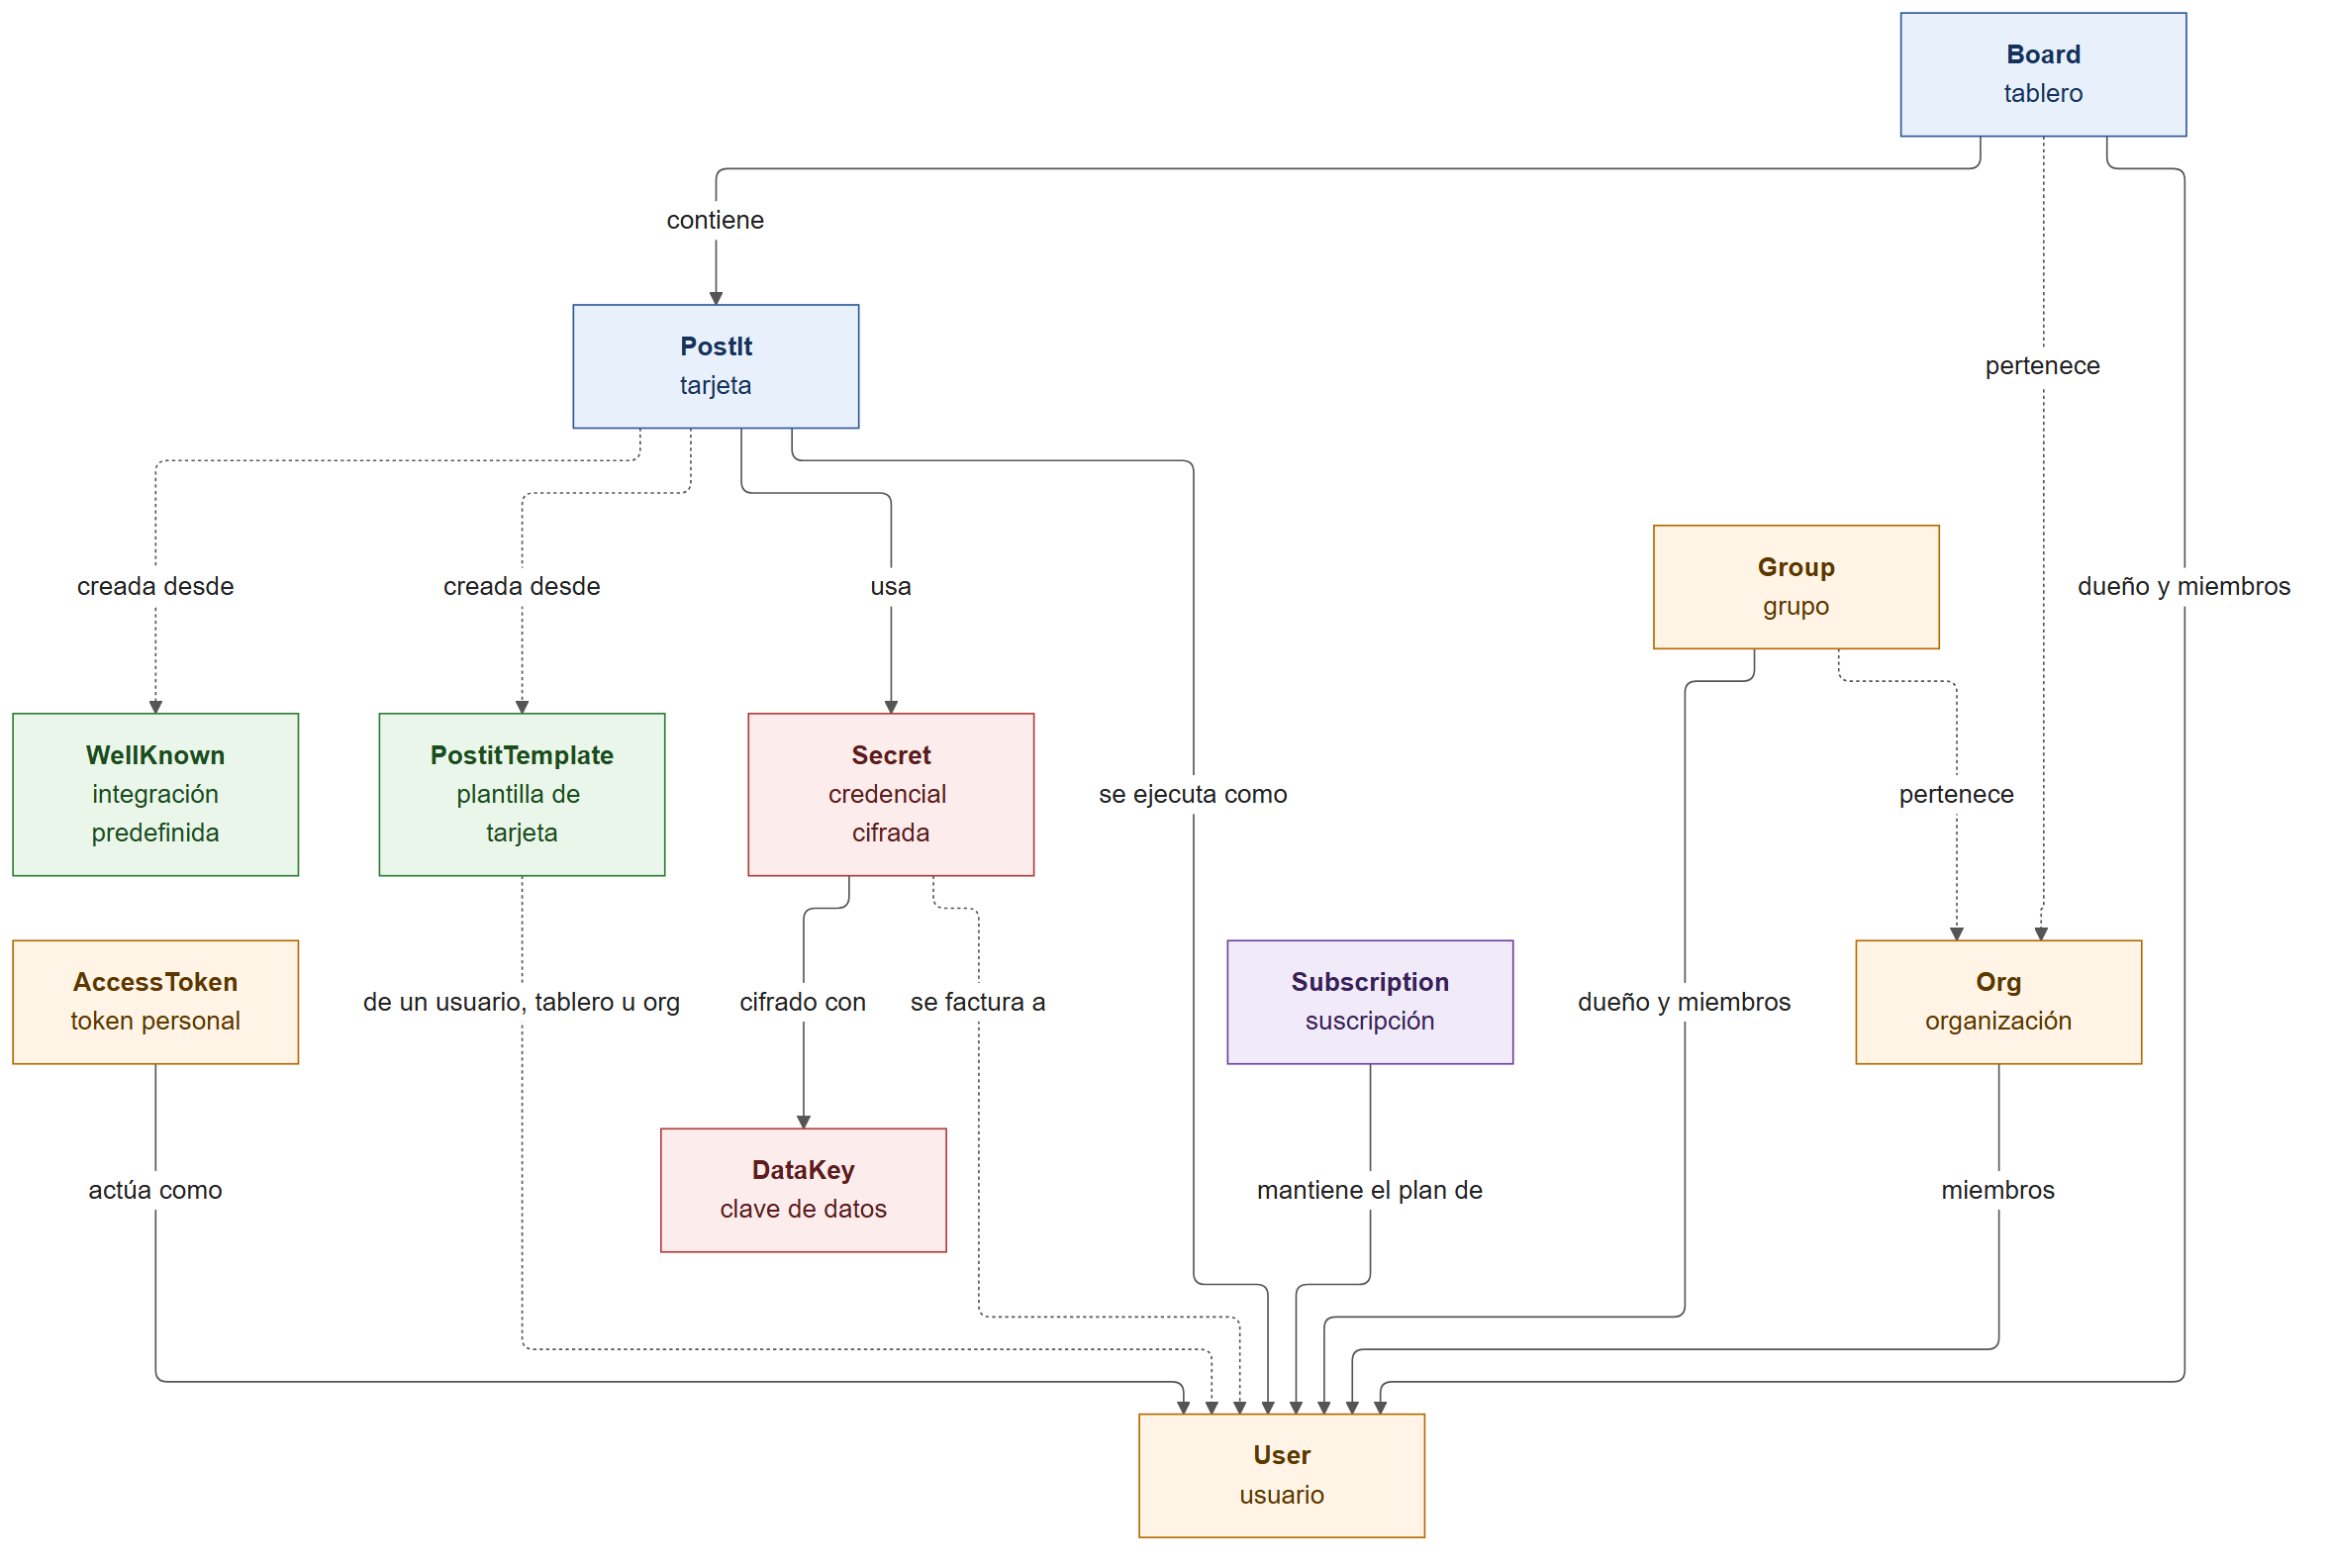
\includegraphics[width=0.95\textwidth]{figuras/fig14.png}
  \caption{Vista general del modelo de dominio}
  \label{fig:modelo_dominio_general}
\end{figure}

\subsection{Tableros y Tarjetas}
La Figura~\ref{fig:modelo_tableros_tarjetas} a continuación detalla el área de tableros, en la cual el tablero embebe a sus miembros con su rol, la posición de cada tarjeta en el lienzo (\texttt{BoardPostIt}) y los hilos que las unen (\texttt{Strand}) con su etiqueta, flechas, grosor y color opcionales, mientras que la configuración de cada tarjeta se guarda en la colección \texttt{postit} con el mismo identificador. Esta separación hace que mover una tarjeta o dibujar un hilo modifique solo el documento del tablero, que es el que observa el servicio de tiempo real.

\begin{figure}[H]
  \centering
  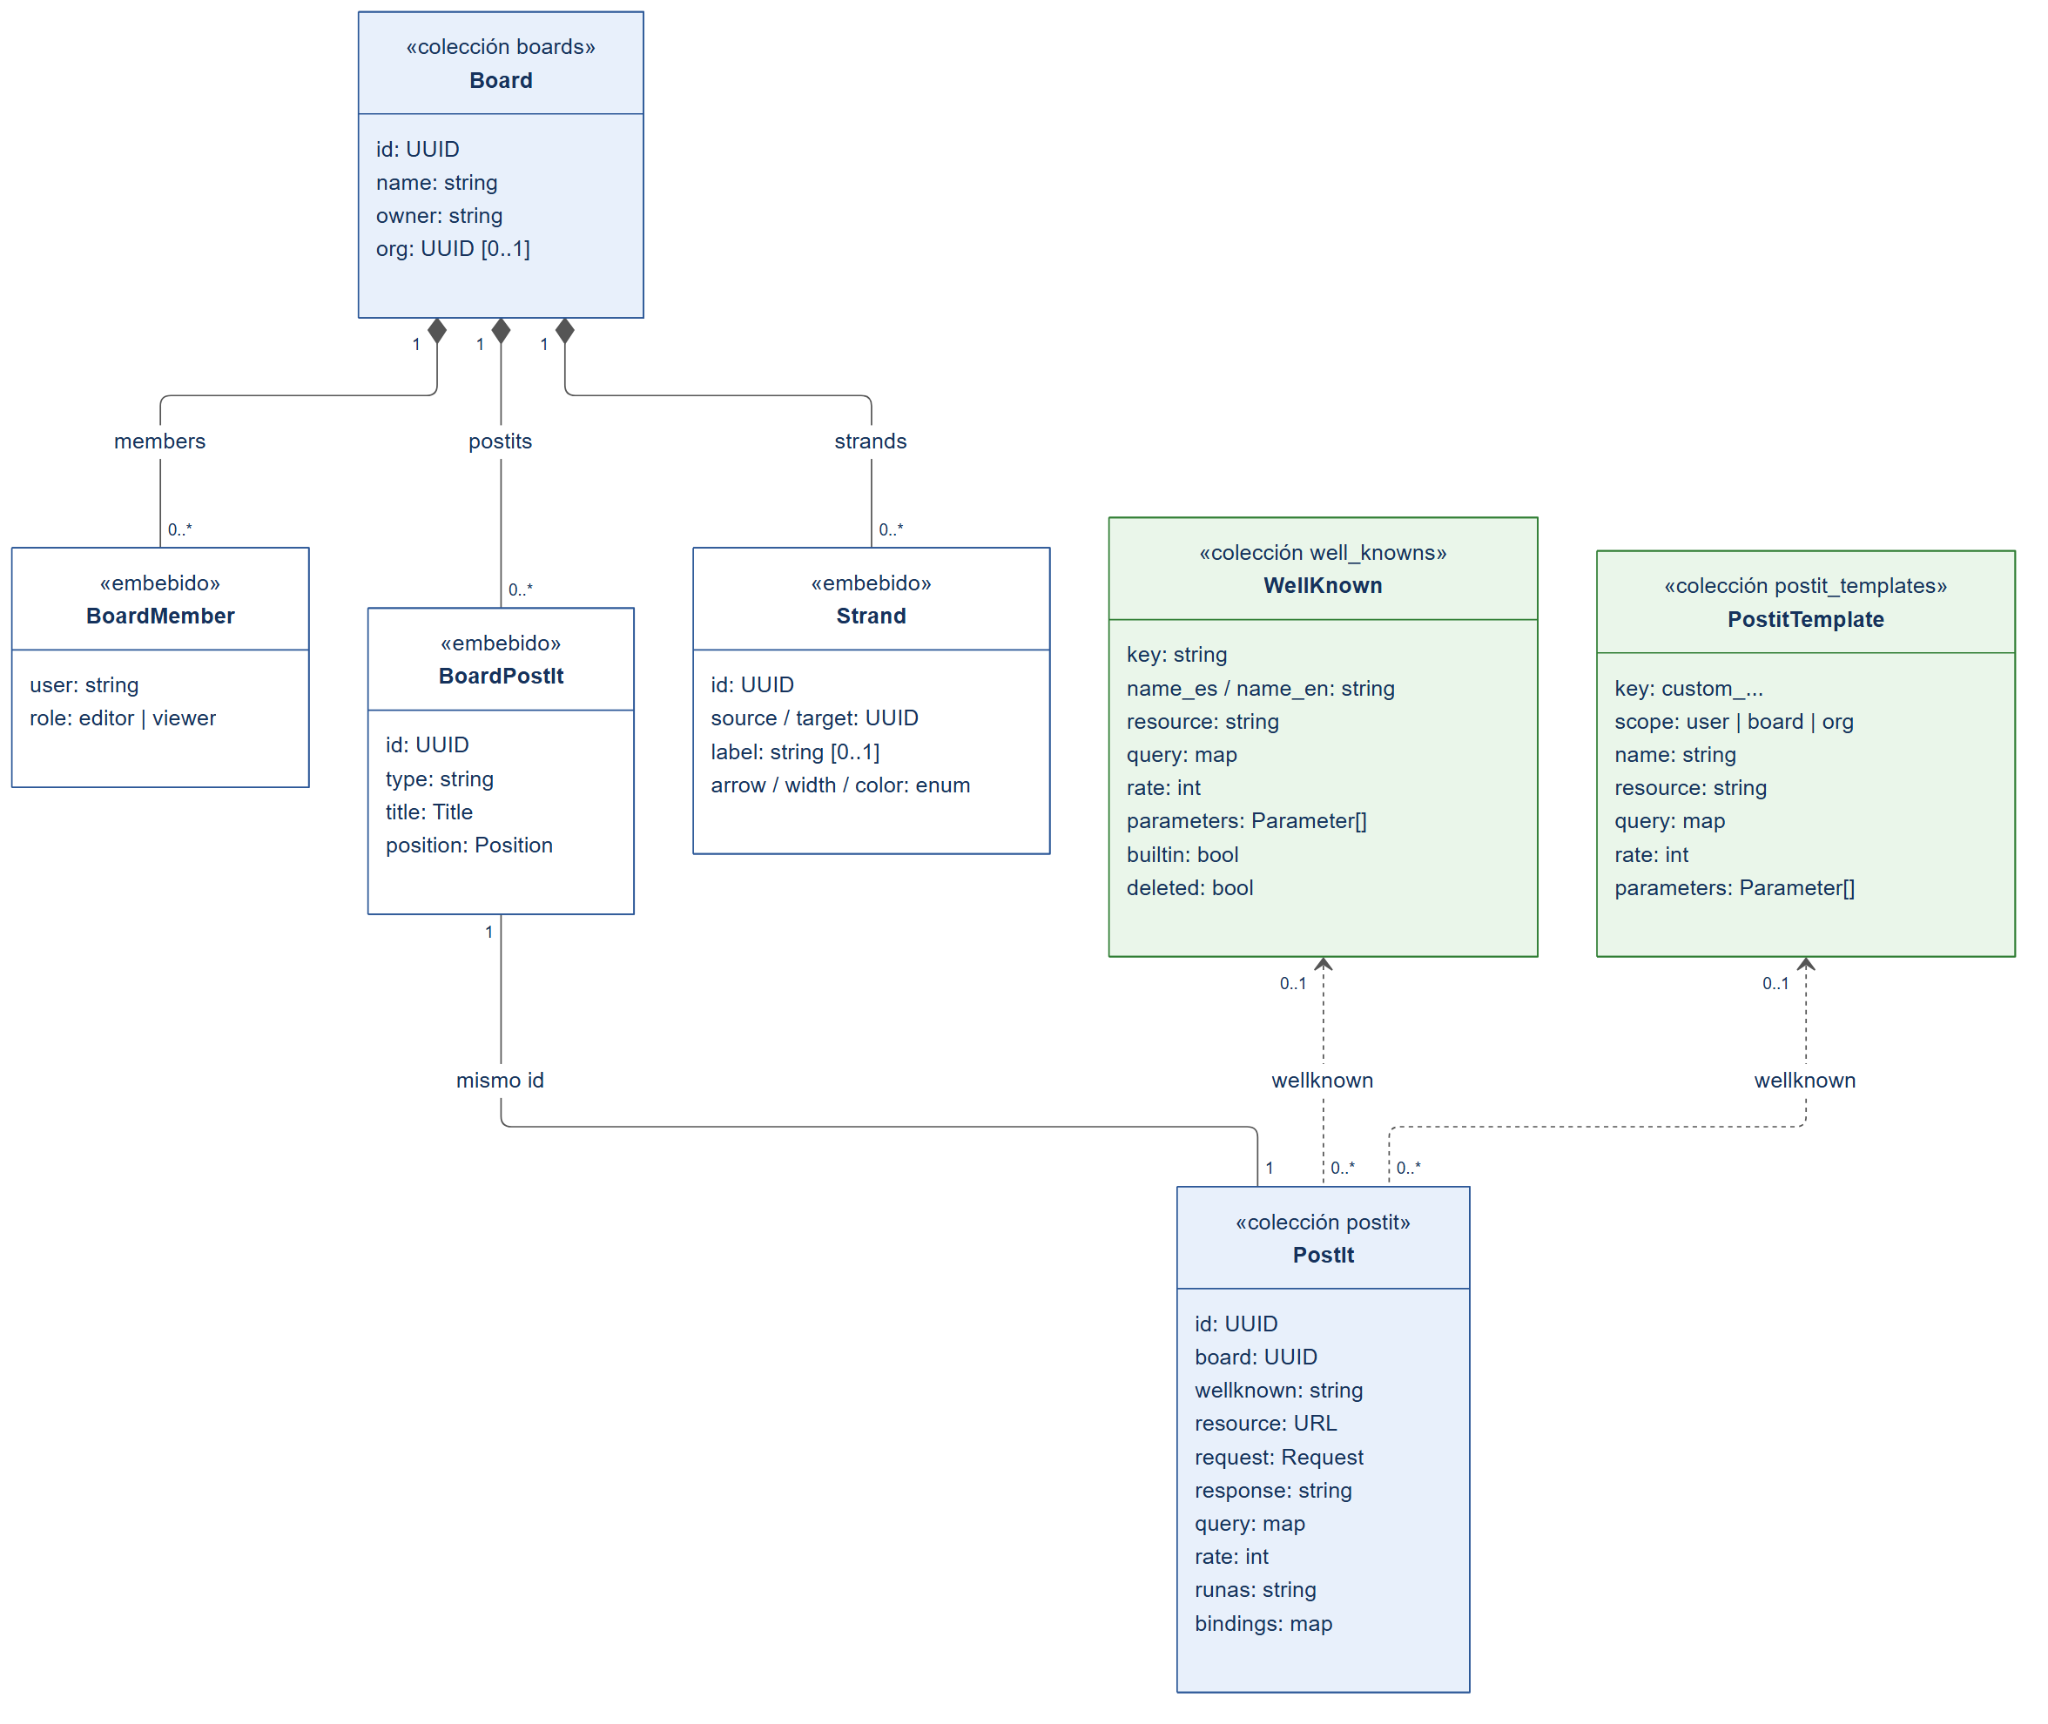
\includegraphics[width=0.95\textwidth]{figuras/fig15.png}
  \caption{Modelo de tableros y tarjetas}
  \label{fig:modelo_tableros_tarjetas}
\end{figure}

\subsection{Identidad y Organizaciones}
El área de identidad se detalla en la Figura~\ref{fig:modelo_identidad}, en la cual cada usuario tiene una o más identidades (contraseña con hash argon2id o cuenta de Google) y puede crear tokens personales, de los que solo se guarda el hash. Las organizaciones listan a sus miembros con rol de administrador o miembro, y los grupos tienen un dueño, una lista de miembros y pueden pertenecer a una organización.

\begin{figure}[H]
  \centering
  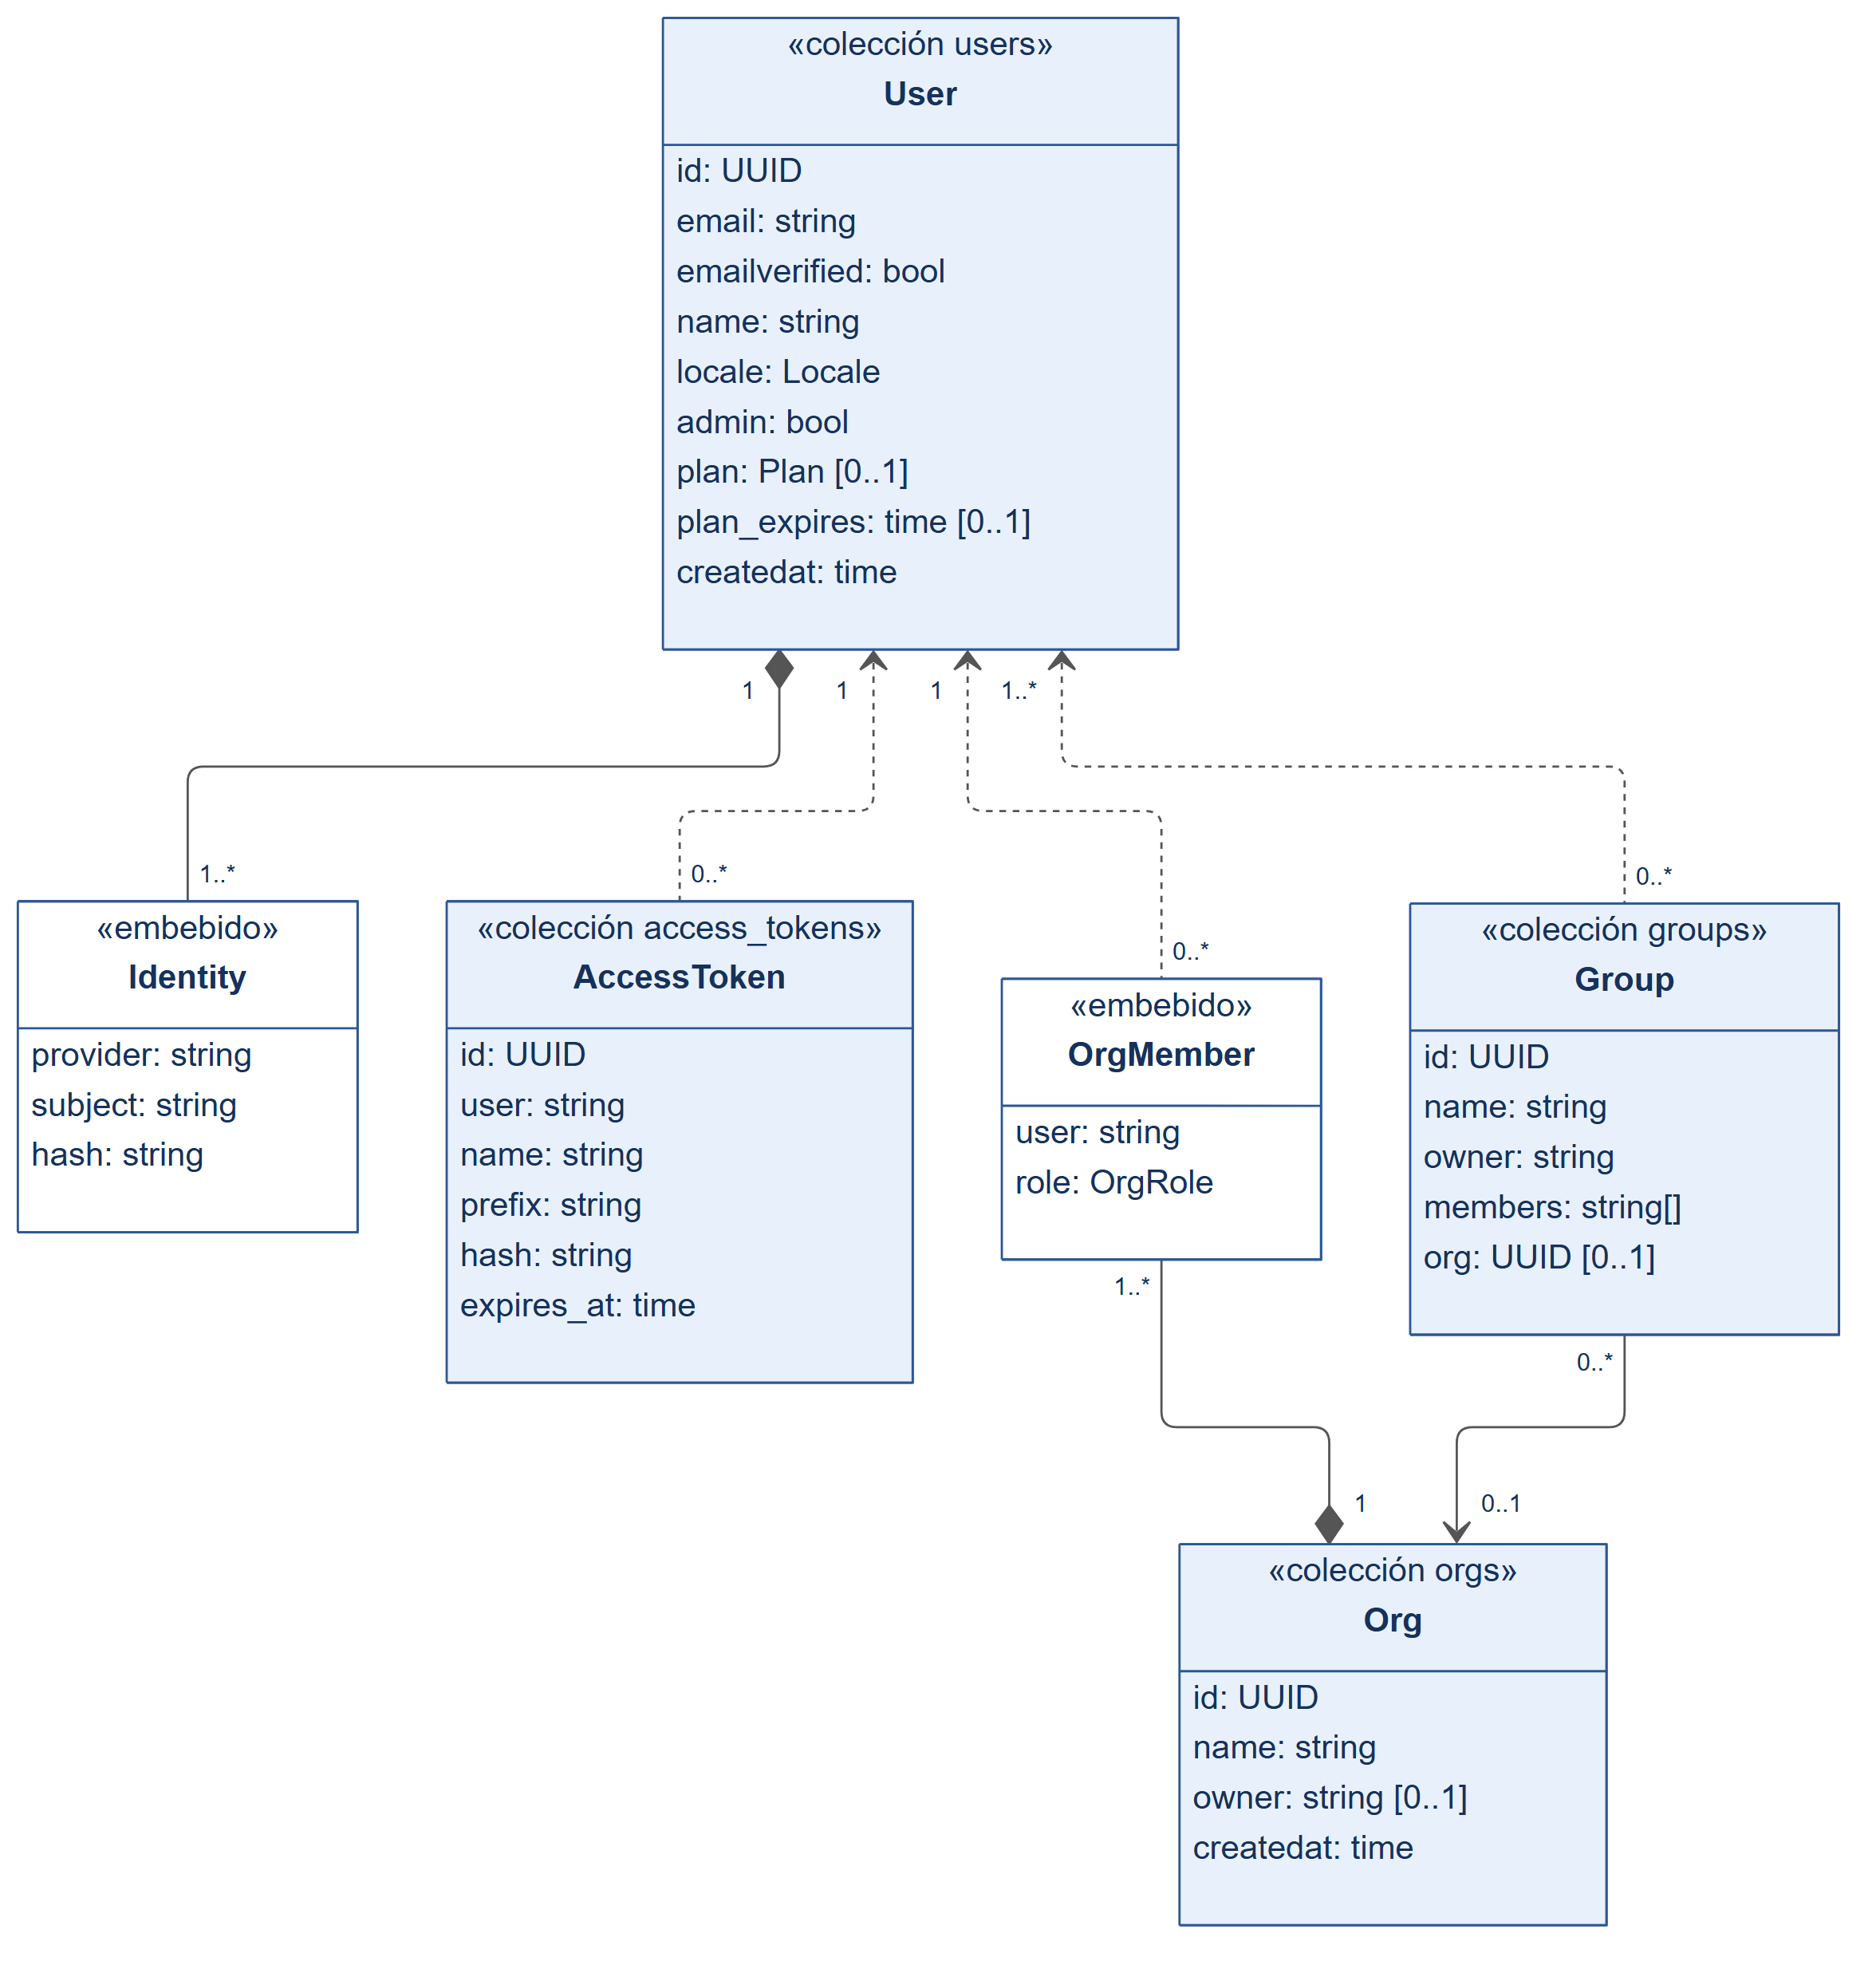
\includegraphics[width=0.92\textwidth]{figuras/fig16.png}
  \caption{Modelo de identidad y organizaciones}
  \label{fig:modelo_identidad}
\end{figure}

\subsection{Bóveda de secretos}
La Figura~\ref{fig:modelo_boveda} muestra el área de la bóveda, en la cual cada tarjeta referencia sus credenciales por ámbito y nombre (\texttt{SecretRef}), sin copiar su valor. Cada secreto se cifra con AES-GCM usando la clave de datos de su ámbito (\texttt{DataKey}), que a su vez se guarda envuelta por la clave maestra versionada, y puede compartirse mediante permisos (\texttt{Grant}) dirigidos a un usuario, un grupo o un tablero.

\begin{figure}[H]
  \centering
  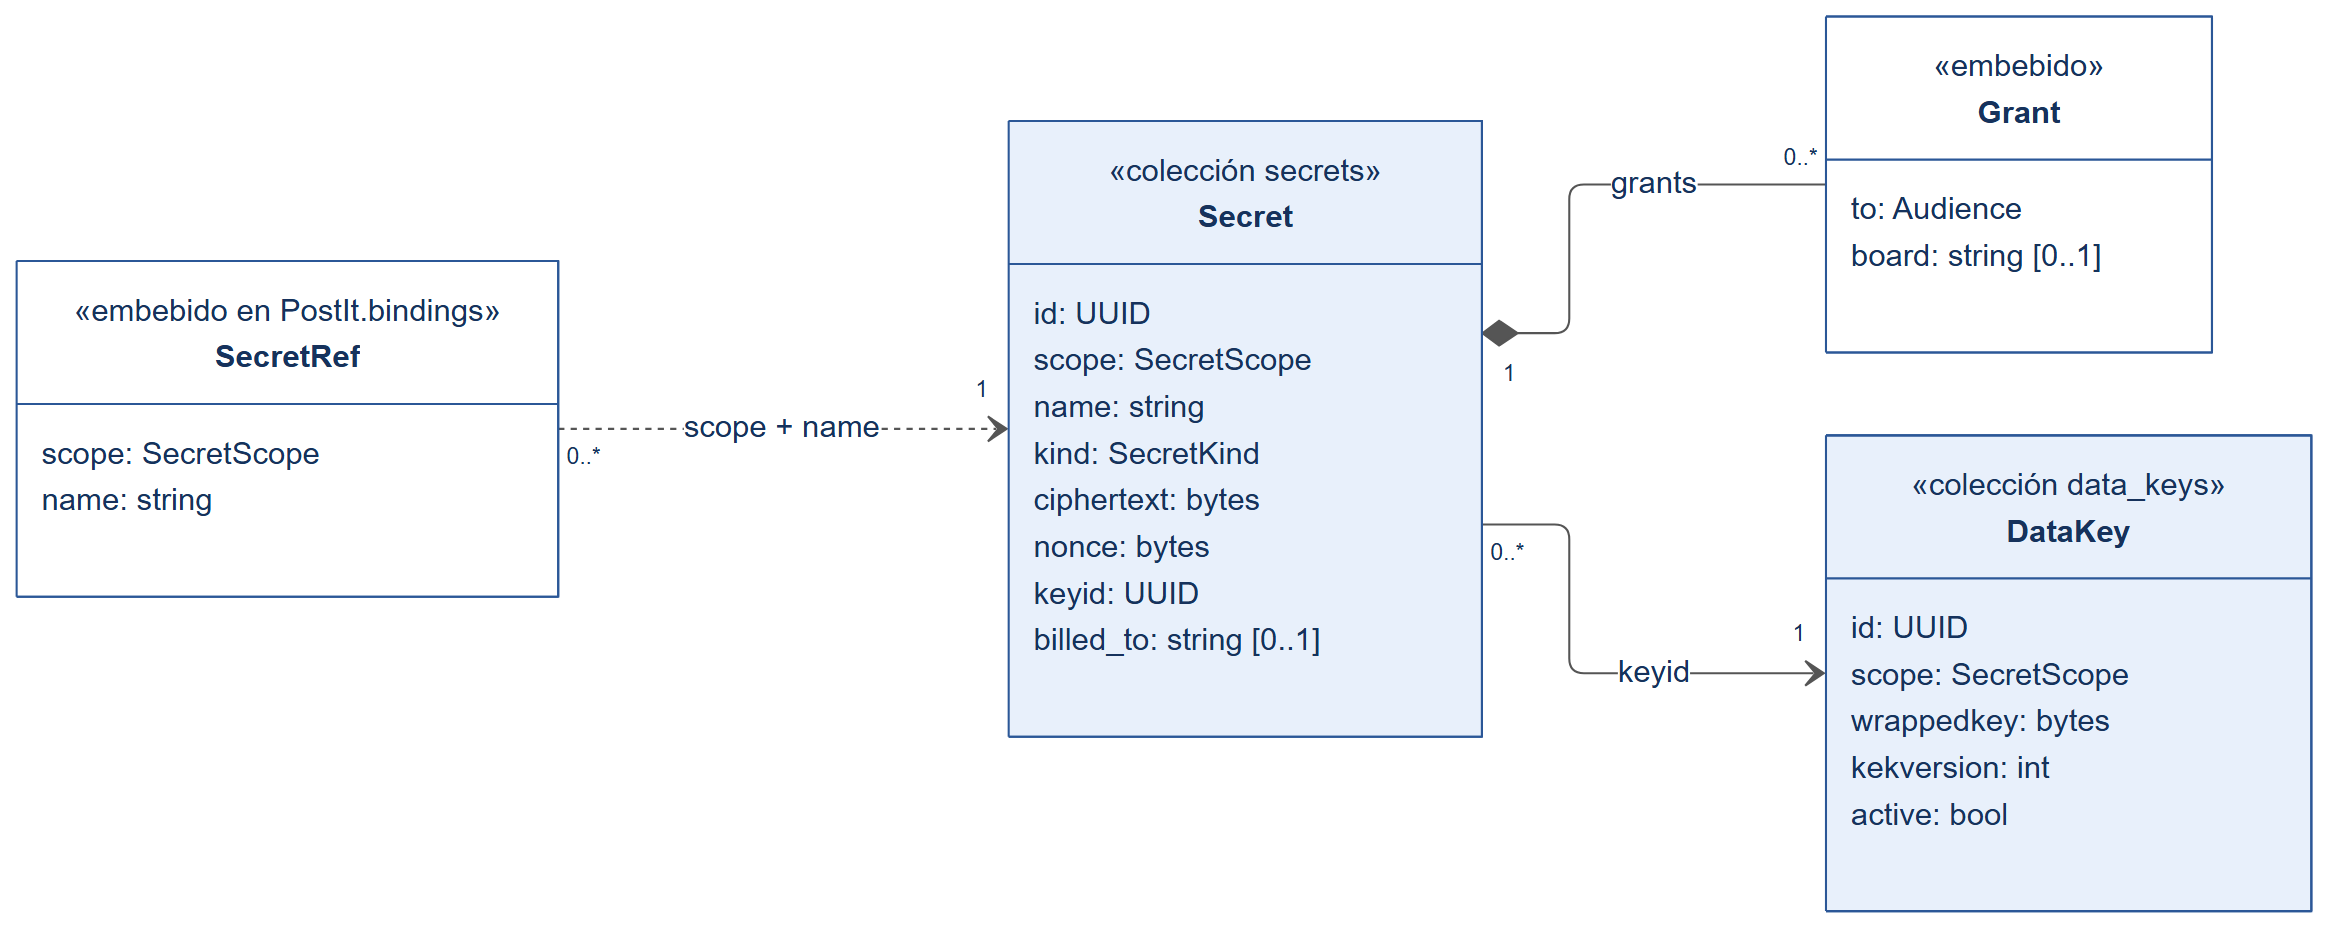
\includegraphics[width=0.95\textwidth]{figuras/fig17.png}
  \caption{Modelo de la bóveda de secretos}
  \label{fig:modelo_boveda}
\end{figure}

\subsection{Planes y suscripciones}
Por último, cada usuario tiene un plan (\texttt{free}, \texttt{pro} o \texttt{max}) con una fecha de vencimiento opcional, y puede tener suscripciones de Mercado Pago que lo mantienen vigente. Los límites de cada plan forman una única tabla (\texttt{Limits}). Cada recurso limitado se factura a un usuario: un tablero a su dueño o al pagador de su organización (\texttt{Org.owner}), y un secreto al usuario indicado en \texttt{billed\_to}. La combinación de pagador, plan y límites que aplica a un recurso se representa con \texttt{Entitlement}. La Figura~\ref{fig:modelo_planes} muestra estas relaciones.

\begin{figure}[H]
  \centering
  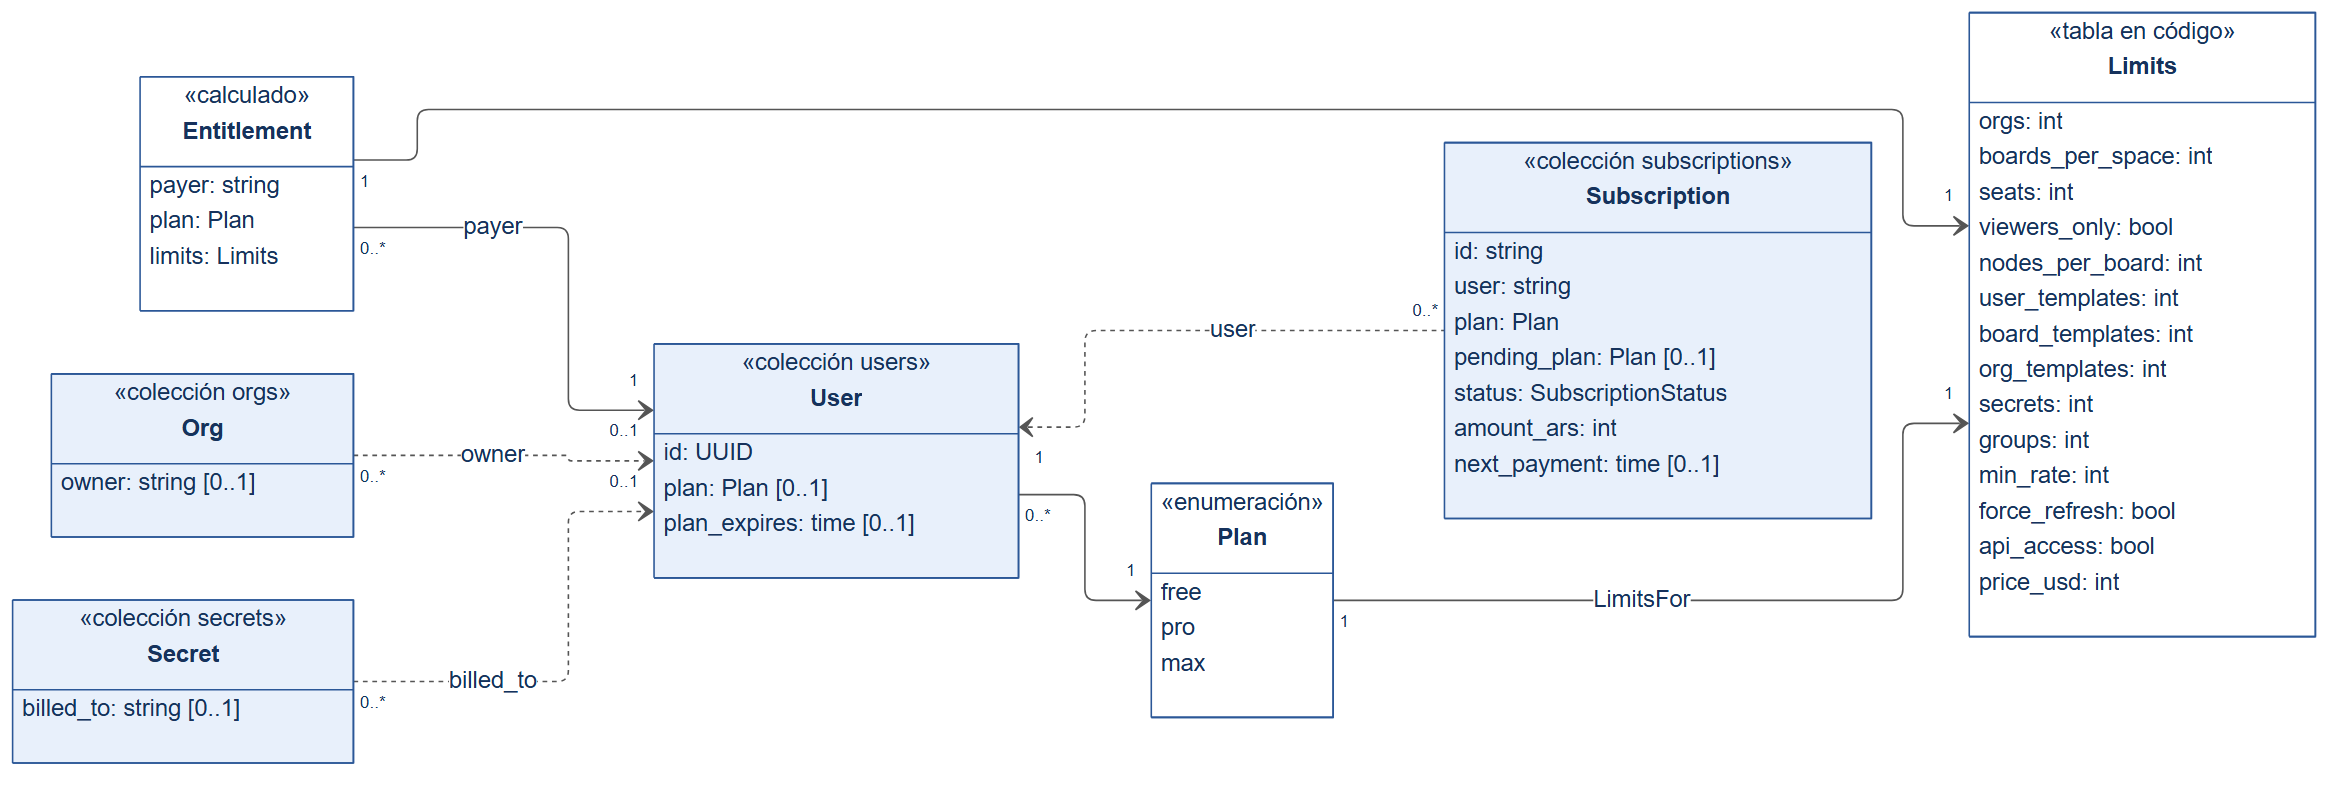
\includegraphics[width=\textwidth]{figuras/fig40.png}
  \caption{Modelo de planes y suscripciones}
  \label{fig:modelo_planes}
\end{figure}

\section{Descripción de sistemas, servicios y plataformas}
A continuación se describe cada componente del sistema, su stack tecnológico, su responsabilidad y la justificación de la elección. Los componentes marcados como planificados forman parte del alcance del proyecto pero no están implementados en el incremento actual.

\begingroup
\footnotesize
\setlength{\tabcolsep}{4.5pt}
\renewcommand{\arraystretch}{1.35}
\rowcolors{2}{gray!7}{white}
\begin{longtable}{
  >{\bfseries\raggedright\arraybackslash}p{\dimexpr 0.16\textwidth - 2\tabcolsep\relax}
  >{\raggedright\arraybackslash}p{\dimexpr 0.24\textwidth - 2\tabcolsep\relax}
  >{\raggedright\arraybackslash}p{\dimexpr 0.30\textwidth - 2\tabcolsep\relax}
  >{\raggedright\arraybackslash}p{\dimexpr 0.30\textwidth - 2\tabcolsep\relax}
}
  \toprule
  \rowcolor{gray!18}
  \textbf{Componente} & \textbf{Tecnología} & \textbf{Responsabilidad} & \textbf{Justificación} \\
  \midrule
  \endfirsthead
  \toprule
  \rowcolor{gray!18}
  \textbf{Componente} & \textbf{Tecnología} & \textbf{Responsabilidad} & \textbf{Justificación} \\
  \midrule
  \endhead
  \midrule
  \rowcolor{white}
  \multicolumn{4}{r}{\textit{\scriptsize Continúa en la página siguiente...}} \\
  \endfoot
  \bottomrule
  \caption{Descripción de componente, la tecnología y la justificación}
  \label{tab:componentes_stack}
  \endlastfoot
  Frontend (SPA) & SvelteKit 2.63 + Svelte 5.56 \cite{svelte_docs}, TailwindCSS 4.3 \cite{tailwind_docs}, TypeScript 6.0 \cite{typescript_docs}, Vite 8.0 \cite{vite_docs}, XyFlow 1.6 \cite{xyflow_docs} & Renderizado del tablero tipo lienzo, manipulación de tarjetas e hilos, edición de configuración y polling de datos a través de la API. & Bundle final pequeño y SSR/SSG opcional, ideal para una interfaz altamente interactiva. Svelte 5 (runes) simplifica el estado reactivo del canvas. \\
  API REST (Backend) & Go 1.27.1 + Gin 1.12 \cite{gin_docs} & Exponer los endpoints bajo \texttt{/api/v1} (auth, users, tokens, boards, post-its, well-knowns, postit-templates, groups, orgs, secrets, billing, system); orquestar autenticación, autorización, persistencia, caché y ejecución de integraciones. & Go aporta concurrencia sencilla (goroutines), tipado estático y binarios pequeños para Docker. Gin se eligió por madurez, middleware y bajo overhead. \\
  Motor de integraciones (Executer) & Go + \texttt{net/http} + \texttt{itchyny/gojq} 0.12 \cite{gojq_docs} + \texttt{PuerkitoBio/goquery} 1.12 \cite{goquery_docs} & Resolver parámetros, ejecutar la petición HTTP, parsear el JSON o HTML y aplicar una expresión jq o jquery para extraer el subconjunto que la tarjeta muestra. & \texttt{gojq} y \texttt{goquery} permiten describir la proyección de datos con sintaxis declarativa estándar, evitando código ad-hoc por integración. Corre con límites (10s y 2MB por petición, hasta 3 redirecciones, 250ms por query). \\
  Base de datos principal & MongoDB 8 \cite{mongodb_docs}, replica set de un nodo & Persistencia de usuarios, tableros, tarjetas, hilos, organizaciones, grupos, la bóveda de secretos y sus claves, tokens personales, el catálogo de integraciones, las plantillas de tarjeta y las suscripciones (11 colecciones, Tabla~\ref{tab:col_boards} y siguientes). & El dominio es naturalmente documental: cada post-it tiene un esquema variable según su integración. Un store relacional implicaría JOINs y normalizaciones sin valor agregado. \\
  Caché de resultados & Redis 7.4 \cite{redis_docs} & Cachear el último resultado de cada post-it, almacenar las sesiones de refresco, los límites de tasa, los locks distribuidos, los handshakes OAuth2 y la presencia por tablero. & TTL nativo por clave que mapea al modelo de tarjeta con su propio refresh rate. Sus operaciones atómicas sirven además para los límites de tasa, los locks distribuidos y la presencia por tablero. \\
  Reverse proxy / ALB & Nginx \cite{nginx_docs} (\texttt{stable-alpine}) & Terminación HTTP en el puerto 80; ruteo de \texttt{/api/*} al backend, de \texttt{/ws/*} al servicio de tiempo real, de \texttt{/mcp} al servidor MCP y del resto al frontend. & Un único entrypoint público que simplifica CORS al servir front y back desde el mismo origen. \\
  Autenticación & Go: \texttt{argon2id} \cite{rfc9106} 1.0, \texttt{golang-jwt} 5.3 \cite{rfc7519} con EdDSA (Ed25519) \cite{rfc8032}, \texttt{go-oidc} 3.21 \cite{oidc_core} para Google & Registro con verificación de correo, login local y con Google, sesiones con token de acceso de 15 minutos y refresh token rotativo en cookie httpOnly. & Una implementación propia evita depender de un proveedor externo y mantiene el mismo flujo en Docker y en Vercel. \texttt{argon2id} es el algoritmo recomendado por OWASP \cite{owasp_password} para contraseñas. \\
  Correo transaccional & Resend \cite{resend_docs} (\texttt{resend-go} 4.8) + plantillas embebidas & Enviar los correos de verificación de cuenta y recuperación de contraseña en el idioma del destinatario. & API simple y de bajo costo; sin clave configurada los correos se vuelcan al log, lo que simplifica el desarrollo local. \\
  Bóveda de secretos & Go: AES-256-GCM \cite{nist_gcm} con envelope encryption & Almacenar credenciales por ámbito (tablero, miembro, usuario, grupo, sistema), resolverlas al ejecutar una tarjeta y gestionar conexiones OAuth2. & El cifrado por sobre (una clave de datos por ámbito envuelta por una clave maestra versionada) permite rotar claves sin recifrar todos los valores. \\
  Planes y facturación & Go + SDK oficial de Mercado Pago (\texttt{mercadopago/sdk-go} 1.14) \cite{mercadopago_docs} & Definir los límites de cada plan, decidir quién paga cada recurso, rechazar con 402 las creaciones que excedan el plan y cobrar las suscripciones mensuales, sincronizándolas mediante webhooks. & Una única tabla de límites en el código evita reglas dispersas. Si no hay credenciales configuradas, la facturación se apaga sin afectar el resto del sistema. \\
  Conector MCP & Servidor MCP en Node.js 24 con \texttt{xmcp} 1.7, que consume la API REST del backend & Exponer tableros y tarjetas a clientes MCP (Claude Desktop, IDEs) para RF-10 y la fase final del cronograma mediante 11 herramientas que presentan cada tablero como un grafo de memorias del agente. & Reutiliza la API REST ya validada y sus reglas de autorización; el servidor MCP es una segunda fachada sobre los mismos casos de uso y no almacena datos propios. Requiere un plan pago (\texttt{api\_access}). \\
  Servicio de tiempo real & Node.js 24 + TypeScript 6.0 + \texttt{socket.io} 4.8 \cite{socketio_docs} & Notificar a cada usuario conectado los cambios de un tablero y mantener la presencia de los participantes. & Los change streams de MongoDB y \texttt{socket.io} permiten propagar cambios sin polling. Separarlo del backend aísla las conexiones persistentes de la API stateless. \\
\end{longtable}
\endgroup
